\chapter{粒子、場、相対論的表記}

\section{講義前のドップラー効果の問題}

前週から持ち越された質問が議論の口火を切る。光速に近い速度で運動する観測者は、常により長い波長を測定するのだろうか。否、答えは運動の向きに依存する。光波と同じ向きに運動する観測者はその波長が引き伸ばされるのを見るのに対し、光波に逆らって運動する観測者はそれが圧縮されるのを見る。これが相対論的ドップラー効果である。

\begin{classroomqa}
\audiencequestion{光速に近い運動は観測される波長を長くするのか。}
\lecturerresponse{観測者が光と同じ向きに運動する場合に限られる。観測者の速度を逆にすればシフトも逆になる。この結果は、別個の公式を暗記することなく、ローレンツ幾何学から直接得ることができる。\lecturetimestamp{00:00:13}}
\end{classroomqa}

\(c=1\)とする単位を用い、プライム付きの系が速さ\(v\)で右へ運動するとする。右向きに進む光の波頭はヌル線に沿う。プライムなしの波長を1に規格化し、連続する二つの波頭の世界線を
\begin{equation}
x=t,
\qquad
x=t+1.
\label{eq:sr5-crest-lines}
\end{equation}
と書く。プライムなしの系における波長は、等しい\(t\)において波頭の間で測定される。プライム付きの系における波長は、代わりに等しい\(t'\)においてそれらの間で測定されなければならない。したがって、同時性の相対性が計算のすべてである。

\begin{figure}[htbp]
\centering
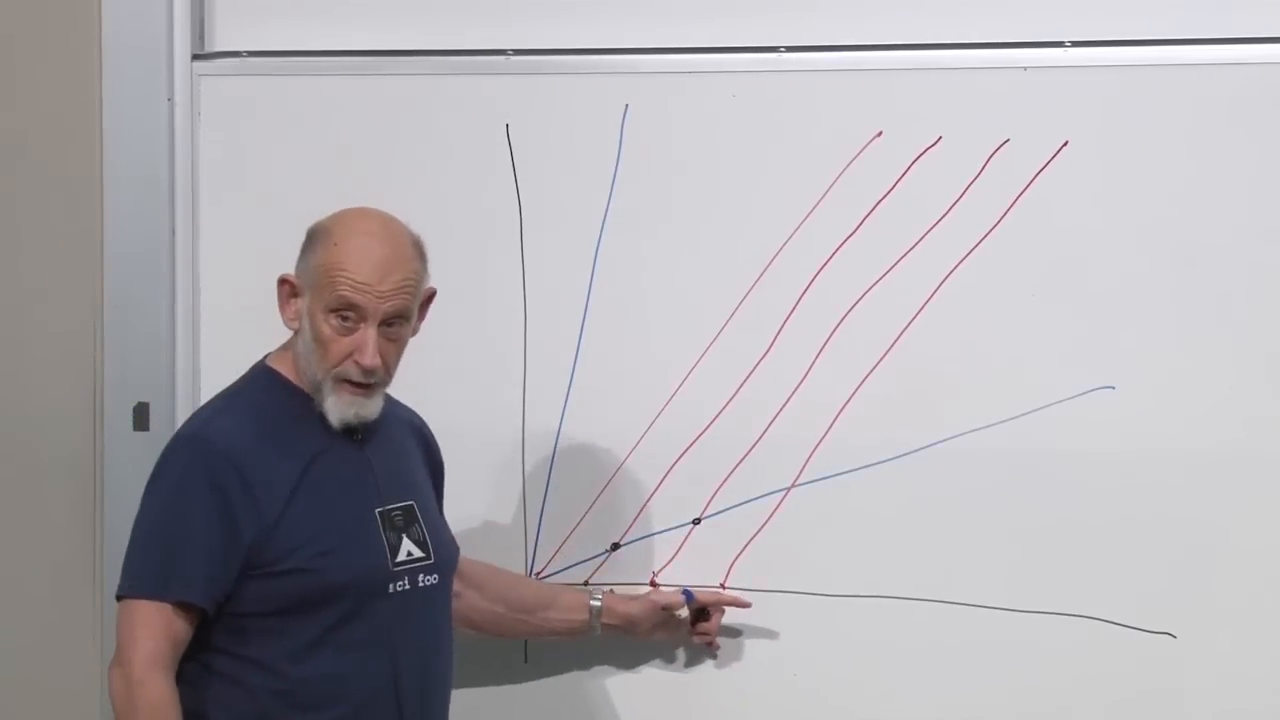
\includegraphics[width=0.90\textwidth]{lecture_05_figure_01.png}
\caption{連続する右向きの波頭、光円錐、および運動する系の傾いた軸。}
\lectureframe{00:03:30}
\end{figure}

ここで導出は、講義の順序についての短い議論のために中断される。夏期講義はない。一般相対性理論と、量子力学へのより広範な回帰が、次の講義の候補である。調和振動子は、量子場の理論の前に理解しておくべき内容として特に挙げられる。

\begin{classroomqa}
\audiencequestion{将来の講義で赤外--紫外の関連を論じることはできるか。}
\lecturerresponse{その問いは量子力学と重力の接点に属する。このクラスにはその問題を認識するのに十分な量子力学があるが、まず重力を、最も自然には一般相対性理論を通じて、発展させなければならない。\lecturetimestamp{00:05:37}}
\end{classroomqa}

\begin{classroomqa}
\audiencequestion{傾いた軸の相対的な目盛りは、単に黒板の図から読み取れるのか。}
\lecturerresponse{否。時空図は因果的および同時性の幾何学を記録するが、図上の通常のユークリッド定規はローレンツ測定ではない。関連する事象を特定し、ローレンツ変換を適用せよ。\lecturetimestamp{00:06:10}}
\end{classroomqa}

ここで計算を再開する。プライムなしの波頭間隔を1に規格化し、プライム付きの系で同時な二つの事象を代数的に特定する。

ローレンツ変換は
\begin{equation}
t'=\gamma(t-vx),
\qquad
x'=\gamma(x-vt),
\qquad
\gamma=\frac{1}{\sqrt{1-v^2}}.
\label{eq:sr5-lorentz-doppler}
\end{equation}
である。プライム付きの同時性の切片\(t'=0\)を選ぶ。すると式\eqref{eq:sr5-lorentz-doppler}より
\begin{equation}
t=vx.
\label{eq:sr5-primed-simultaneity}
\end{equation}
が得られる。最初の波頭はこの切片と原点で交わる。二番目の波頭は\(x=t+1\)に従うので、その交点は
\begin{align}
x&=vx+1,\\
x&=\frac{1}{1-v},
\qquad
t=\frac{v}{1-v}.
\end{align}
を満たす。そのプライム付き座標は
\begin{align}
x'
&=\frac{x-vt}{\sqrt{1-v^2}}\\
&=\frac{1-v^2}{(1-v)\sqrt{1-v^2}}\\
&=\sqrt{\frac{1+v}{1-v}}.
\end{align}
である。元の波長が1であったから、
\begin{equation}
\boxed{
\frac{\lambda'}{\lambda}
=
\sqrt{\frac{1+\beta}{1-\beta}}
},
\qquad
\beta=\frac{v}{c}.
\label{eq:sr5-doppler}
\end{equation}
同値に、
\begin{equation}
\frac{\lambda'}{\lambda}
=
\sqrt{\frac{c+v}{c-v}}.
\end{equation}

\begin{figure}[htbp]
\centering
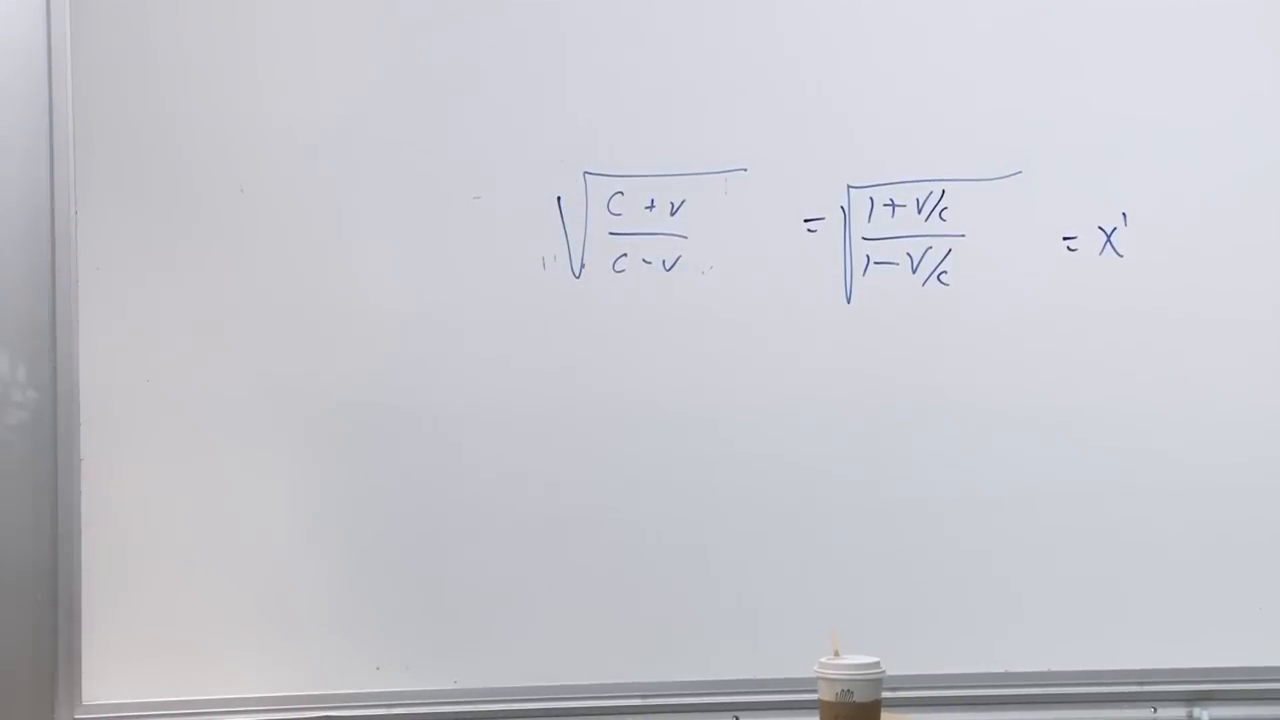
\includegraphics[width=0.90\textwidth]{lecture_05_figure_02.png}
\caption{\(c\)を復元した後のドップラー因子。\(v\)を逆にすると逆数のシフトが得られる。}
\lectureframe{00:13:40}
\end{figure}

\(v>0\)のとき、プライム付きの観測者は光を追いかけ、より長い波長を測定する。\(v\)を\(-v\)に置き換えると、光に逆らう運動を記述し、因子は1より小さくなる。観測者が光線を追いかけながら\(c\)に近づくことができれば、波長は発散するであろう。周波数のシフトは逆比である。

\section{なぜ相互作用は一つの作用に現れなければならないか}

予備的な質問の後、主題は場と粒子である。量子場の理論では、粒子と場は最終的に同じ励起の二つの記述となるであろう。それはここでの枠組みではない。ここでは粒子は世界線に従い、古典場が時空を満たす。当面の問いはより控えめである。すなわち、場が粒子に作用するならば、粒子はどのように場に作用し返すのか。

作用原理はこれを有限次元の原型を通じて答える。\(x(t)\)と\(y(t)\)を二つの一般化座標とする。ラグランジアンが分離するならば、
\begin{equation}
L(x,\dot x,y,\dot y)
=
L_x(x,\dot x)+L_y(y,\dot y),
\label{eq:sr5-separable-l}
\end{equation}
二つのオイラー--ラグランジュ方程式は独立である。
\begin{equation}
\frac{d}{dt}\frac{\partial L}{\partial\dot x}
=
\frac{\partial L}{\partial x},
\qquad
\frac{d}{dt}\frac{\partial L}{\partial\dot y}
=
\frac{\partial L}{\partial y}.
\end{equation}
\(x\)の方程式は\(y\)を含まず、\(y\)の方程式は\(x\)を含まない。

変数を相互作用させるには、\(x\)の部分と\(y\)の部分に分けることのできない項を加える。簡単な例は
\begin{equation}
L
=
\frac{\dot x^2}{2}
+\frac{\dot y^2}{2}
-V(x)-W(y)+\kappa xy.
\label{eq:sr5-coupled-coordinates}
\end{equation}
である。今や\(x\)を変分すると\(y\)に比例する項が生じ、\(y\)を変分すると\(x\)に比例する項が生じる。同じ混合項が影響の両方向を支配する。

\begin{figure}[htbp]
\centering
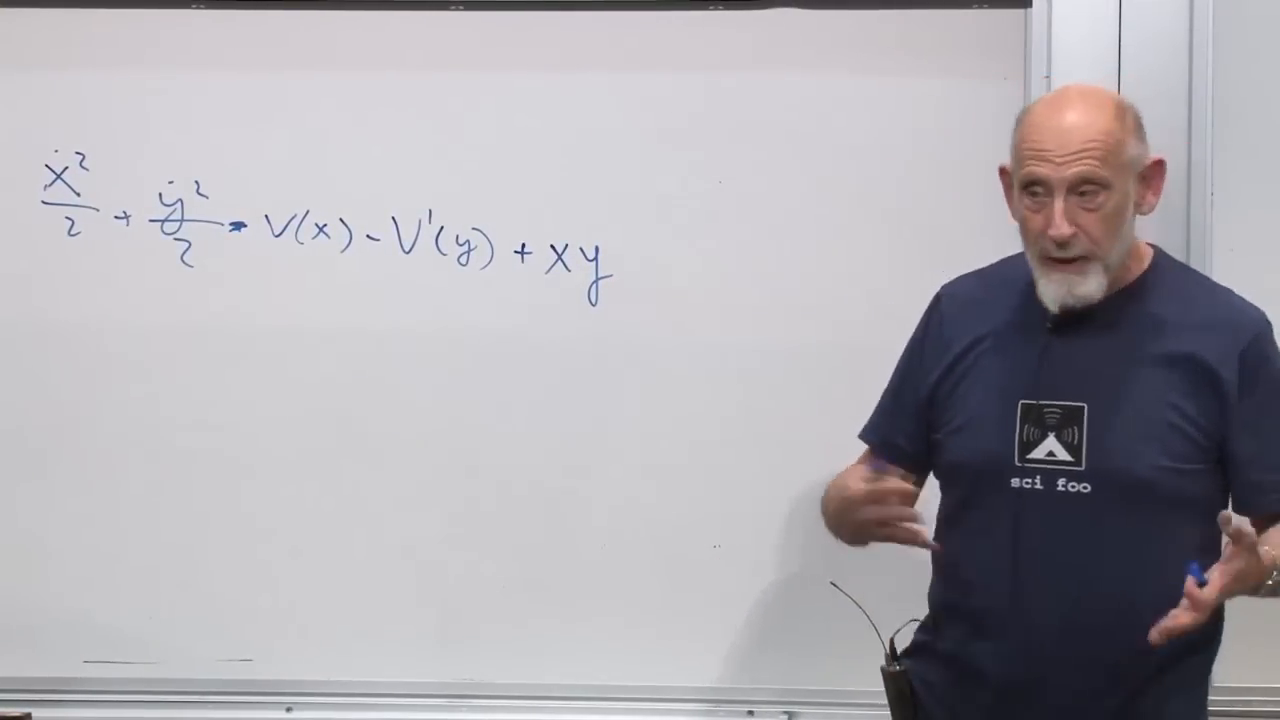
\includegraphics[width=0.90\textwidth]{lecture_05_figure_03.png}
\caption{ラグランジアンの中の一つの項が二つの一般化座標の両方を含むとき、それら二つの一般化座標は動的に結合する。}
\lectureframe{00:19:00}
\end{figure}

これが、ここで用いる作用--反作用の言明の正確な設定である。すなわち、両方の対象が力学的であり、両方が1つの共通の作用において変分される。場を外部から指定された背景として扱うと、その応答が隠れてしまうことがあるが、いったん場自体が力学的になれば、結合項が両方の方程式を与える。

\section{スカラー場が粒子にどのように作用するか}

\subsection{相対論的結合}

まずスカラー場\(\phi(\mathbf{x},t)\)を既知として扱う。それは波であっても静的プロファイルであってもよく、当面はそれ自身の方程式は無関係である。自由相対論的粒子の作用は
\begin{equation}
S_{\mathrm p}
=
-m\int d\tau.
\end{equation}
であり、直線上の運動と\(c=1\)に対して
\begin{equation}
L_{\mathrm p}^{(0)}
=
-m\sqrt{1-\dot x^2}.
\end{equation}
である。最も単純なスカラー結合は、質量の係数を場に依存する係数で置き換える：
\begin{equation}
\boxed{
L_{\mathrm p}
=
-\bigl[m+g\phi(x,t)\bigr]\sqrt{1-\dot x^2}
}.
\label{eq:sr5-particle-coupling}
\end{equation}
結合定数\(g\)は、場がこの粒子にどれほど強く影響するかを測る。その符号は規約であり、\(g\)を\(-g\)に変えるとスカラー力の向きが反転する。

\begin{figure}[htbp]
\centering
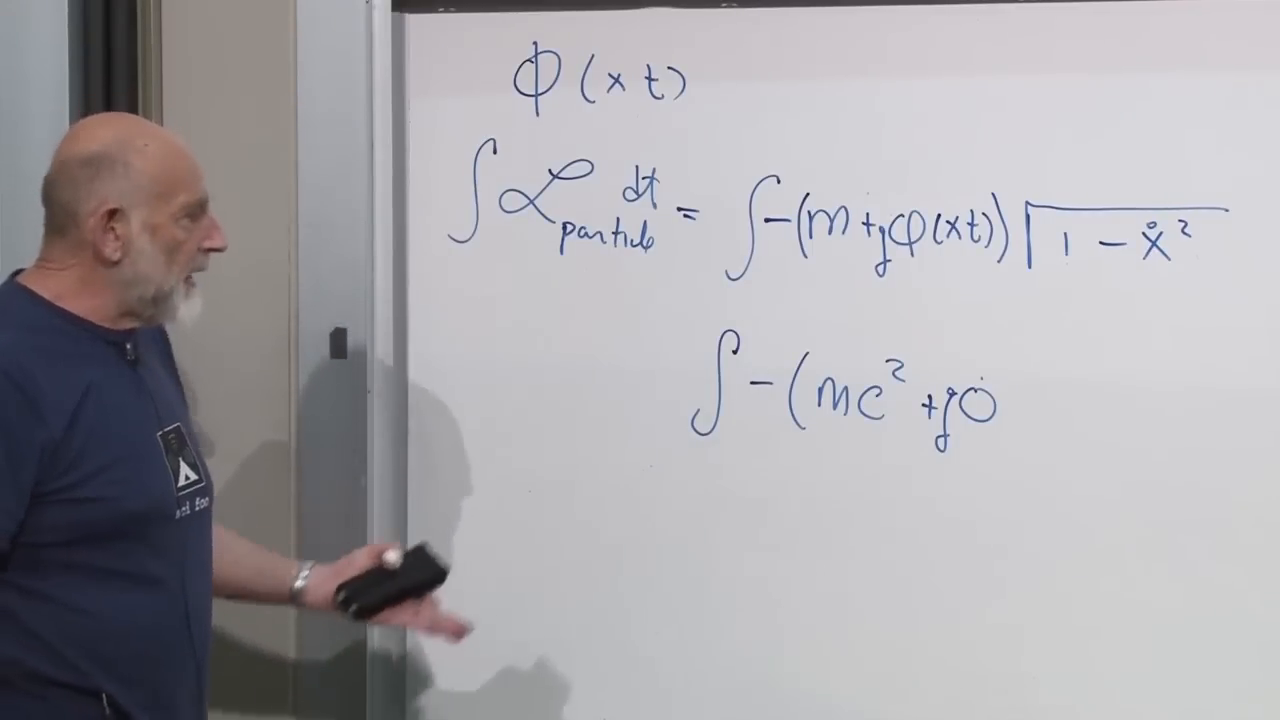
\includegraphics[width=0.90\textwidth]{lecture_05_figure_04.png}
\caption{\(m\)を局所係数\(m+g\phi(x,t)\)で置き換えた自由粒子の作用。}
\lectureframe{00:24:10}
\end{figure}

\subsection{低速粒子極限}

ニュートン極限が見えるように光速を復元する：
\begin{equation}
L_{\mathrm p}
=
-\bigl[mc^2+g\phi(x,t)\bigr]
\sqrt{1-\frac{\dot x^2}{c^2}}.
\label{eq:sr5-particle-coupling-c}
\end{equation}
\(|\dot x|\ll c\)に対して
\begin{equation}
\sqrt{1-\frac{\dot x^2}{c^2}}
=
1-\frac{\dot x^2}{2c^2}
+O\!\left(\frac{\dot x^4}{c^4}\right).
\end{equation}
\eqref{eq:sr5-particle-coupling-c}に代入すると、定数\(-mc^2\)と\(c^{-2}\)で抑制される項を落とした後、
\begin{align}
L_{\mathrm p}
&=
-mc^2-g\phi
+\frac{m\dot x^2}{2}
+\frac{g\phi\,\dot x^2}{2c^2}
+O(c^{-4})\\
&\longrightarrow
\frac{m\dot x^2}{2}-g\phi(x,t),
\label{eq:sr5-nr-particle}
\end{align}
が得られる。結果は通常の形\(T-V\)であるから、
\begin{equation}
V_{\mathrm p}(x,t)=g\phi(x,t).
\label{eq:sr5-scalar-potential}
\end{equation}

\begin{figure}[htbp]
\centering
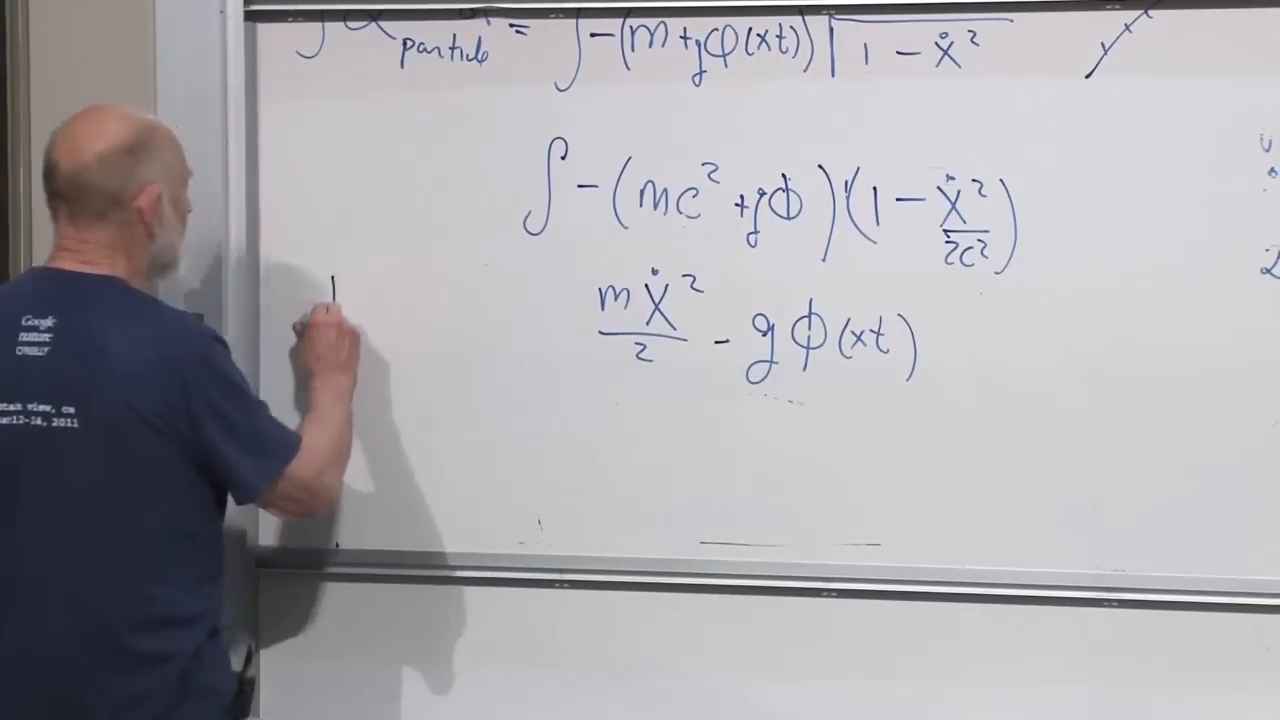
\includegraphics[width=0.90\textwidth]{lecture_05_figure_05.png}
\caption{平方根の展開はニュートン的運動項とスカラーポテンシャルエネルギー\(g\phi\)を残す。}
\lectureframe{00:28:50}
\end{figure}

大きな静止エネルギー定数はオイラー--ラグランジュ方程式には入らない。場に依存する項は入る。電磁気学では、電荷が結合の強さに類似した役割を果たすが、実際の電磁相互作用はこのスカラーの玩具模型ではなく四元ベクトルポテンシャルを用いる。

\section{粒子が場にどのように逆向きに作用するか}

\subsection{1つの変分問題}

もはや場は単に指定されたままとどまることはできない。場の配置と粒子の世界線の両方を含む時空領域を考える。物理的解は、両方の変分の下で全作用を停留させる：
\begin{equation}
\delta S[\phi,x]=0.
\end{equation}
場を固定して世界線を変分すると粒子の方程式が得られる。世界線を固定して場を変分すると場の方程式が得られる。それらを結びつけるのは、両者に共通の相互作用項である。

\begin{figure}[htbp]
\centering
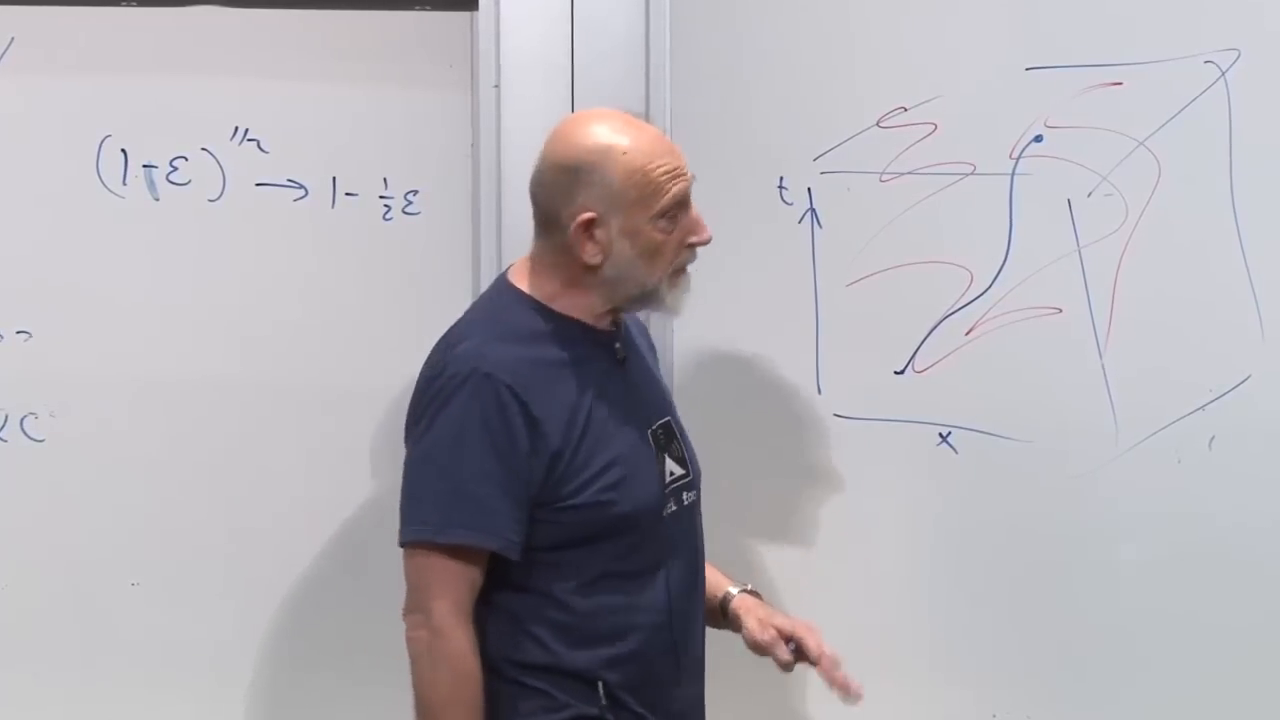
\includegraphics[width=0.90\textwidth]{lecture_05_figure_06.png}
\caption{スカラー場が占める時空領域を通る粒子の世界線。}
\lectureframe{00:30:30}
\end{figure}

自由質量ゼロのスカラー場に対して、
\begin{equation}
S_{\mathrm f}
=
\int d^4x\,
\frac12
\left[
(\partial_t\phi)^2
-(\partial_x\phi)^2
-(\partial_y\phi)^2
-(\partial_z\phi)^2
\right].
\label{eq:sr5-free-field-action}
\end{equation}
をとる。これ以降は再び\(c=1\)を用いる。明示的な単位では、座標と場の規格化に応じて、時間の項は対応する\(1/c^2\)の因子を伴うであろう。

\begin{figure}[htbp]
\centering
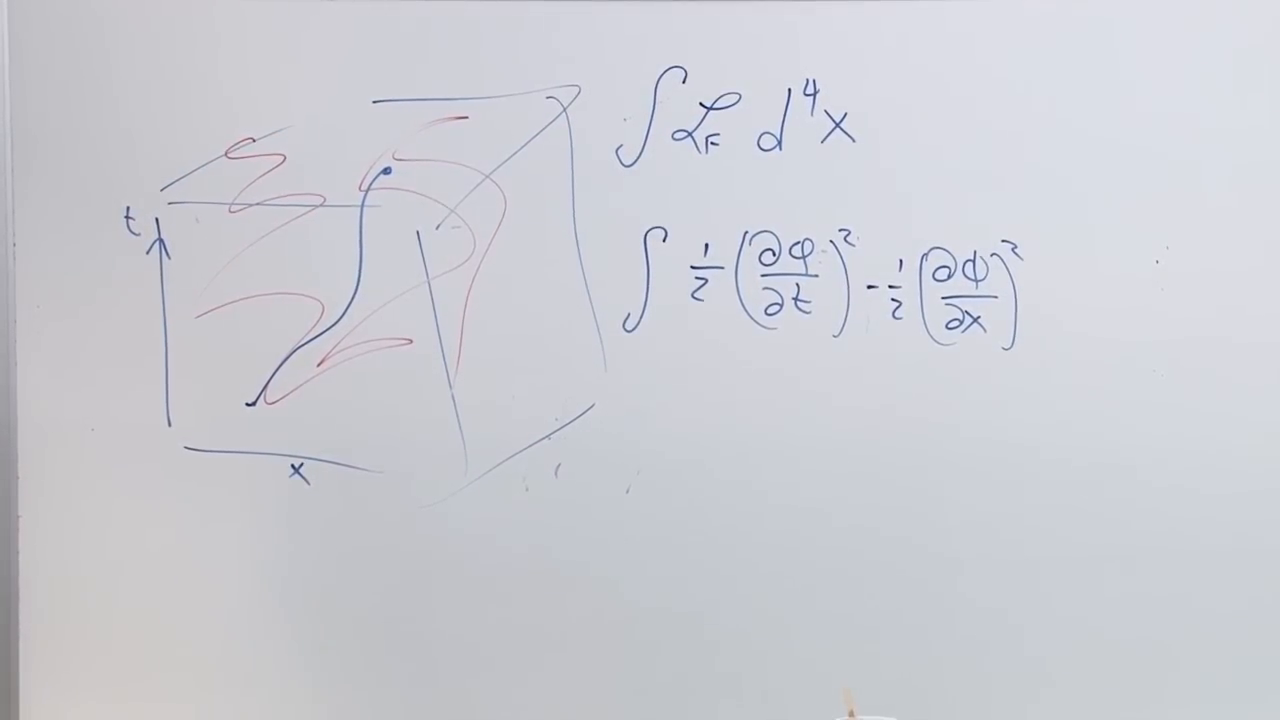
\includegraphics[width=0.90\textwidth]{lecture_05_figure_07.png}
\caption{粒子の世界線と同じ時空領域上で書かれた場の作用。}
\lectureframe{00:32:10}
\end{figure}

\subsection{静的粒子と世界線積分}

最小限の代数で源をあらわにするため、粒子を原点に静止させる。そのとき因子\(d\tau\)は\(dt\)に等しく、\eqref{eq:sr5-particle-coupling}の相互作用部分は
\begin{equation}
S_{\mathrm{int}}
=
-g\int dt\,\phi(\mathbf{0},t).
\label{eq:sr5-worldline-interaction}
\end{equation}
となる。これは世界線に沿った積分にすぎないのに対し、
\eqref{eq:sr5-free-field-action}は全時空にわたる積分である。それらを1つの時空積分にまとめるには、粒子の位置を選び出す関数が必要である。

\begin{figure}[htbp]
\centering
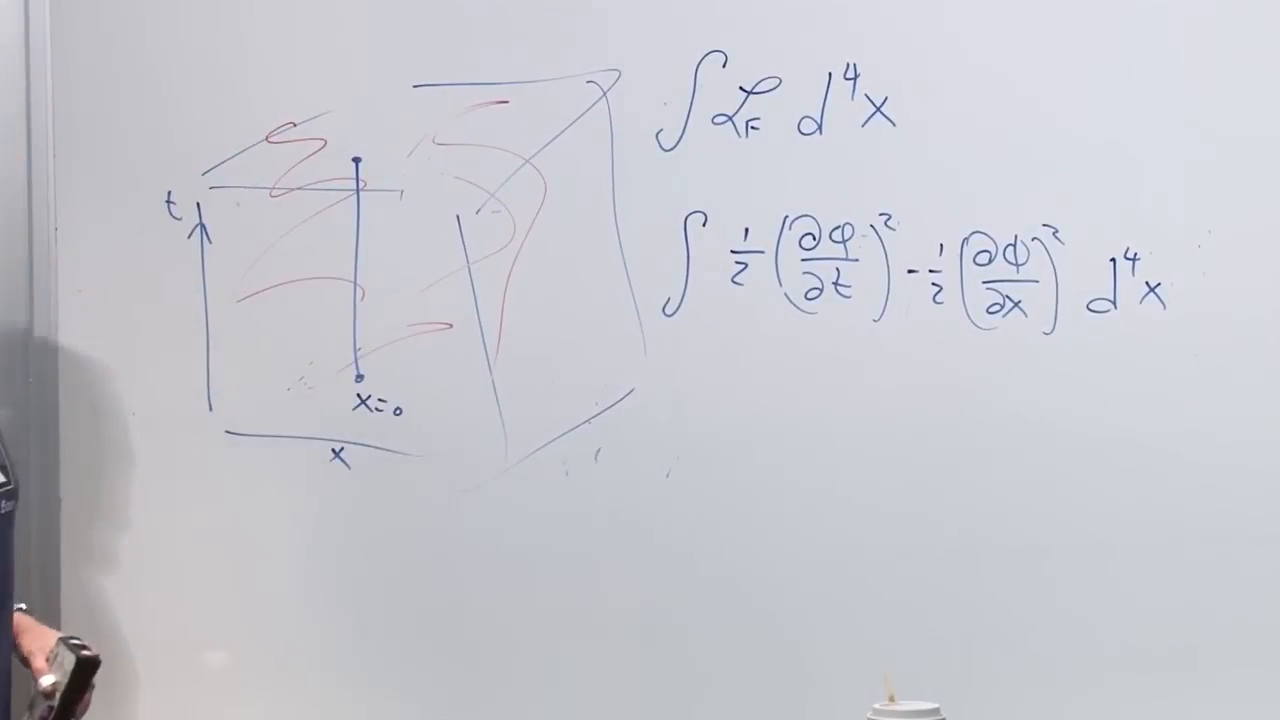
\includegraphics[width=0.90\textwidth]{lecture_05_figure_08.png}
\caption{場の領域内の静的世界線と、それと結合されなければならない場の作用。}
\lectureframe{00:35:35}
\end{figure}

\subsection{ディラックのデルタ関数}

一次元デルタ関数は次で定義される。
\begin{equation}
\int_{-\infty}^{\infty}dx\,f(x)\delta(x-a)=f(a).
\label{eq:sr5-delta-definition}
\end{equation}
これは\(x=a\)から離れると消え、\(x=a\)で特異であり、積分値は一である。
これは通常の有限値関数というよりも、\eqref{eq:sr5-delta-definition}で特徴づけられる超関数として理解するのが最もよい。

\begin{figure}[htbp]
\centering
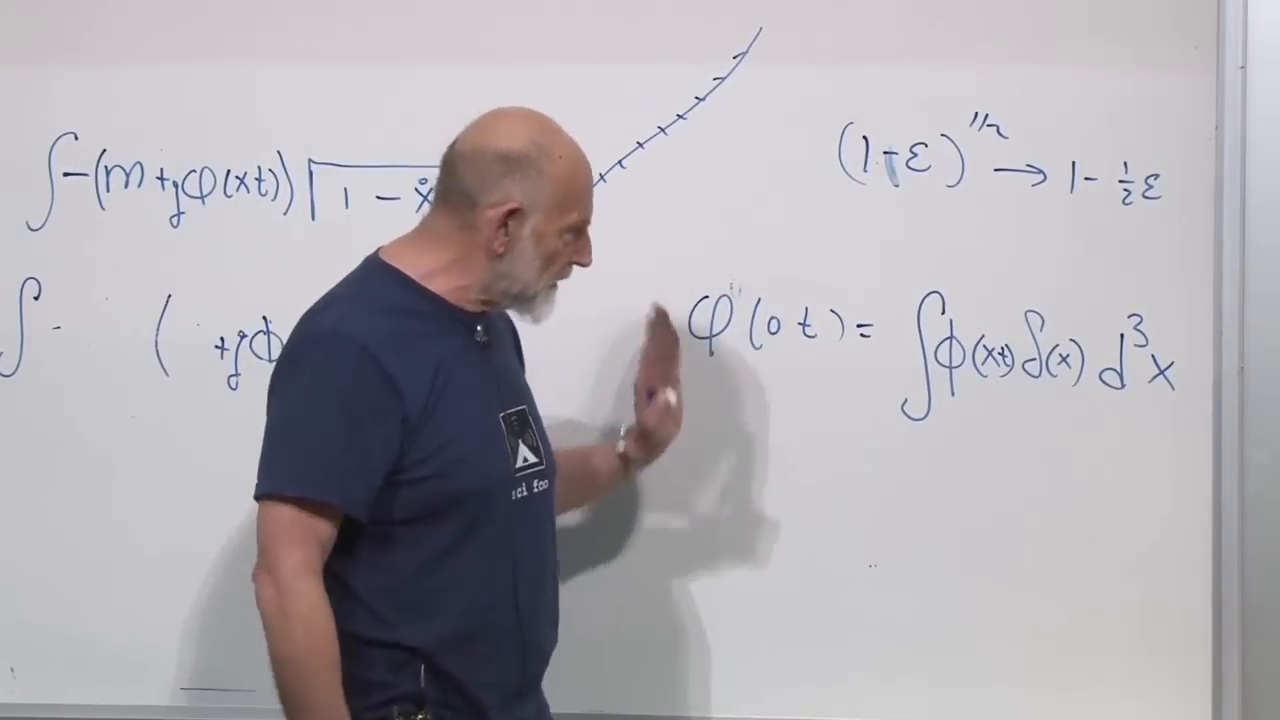
\includegraphics[width=0.90\textwidth]{lecture_05_figure_09.png}
\caption{原点における場の値を空間積分に書き換えるデルタ関数の恒等式。}
\lectureframe{00:36:45}
\end{figure}

3次元では
\begin{equation}
\delta^3(\mathbf{x})
=
\delta(x)\delta(y)\delta(z),
\end{equation}
であり、したがって
\begin{align}
\int d^3x\,
\phi(\mathbf{x},t)\delta^3(\mathbf{x})
&=
\int dx\,dy\,dz\,
\phi(x,y,z,t)\\
&\quad\times\delta(x)\delta(y)\delta(z)\\
&=\phi(\mathbf{0},t).
\label{eq:sr5-triple-delta}
\end{align}

\begin{classroomqa}
\audiencequestion{\(d^3x\)はどこから来るのか。}
\lecturerresponse{それは通常の空間体積要素\(dx\,dy\,dz\)である。1つの空間次元では、同じ恒等式は\(dx\)と1つのデルタ関数のみを含む。\lecturetimestamp{00:37:09}}
\end{classroomqa}

\begin{figure}[htbp]
\centering
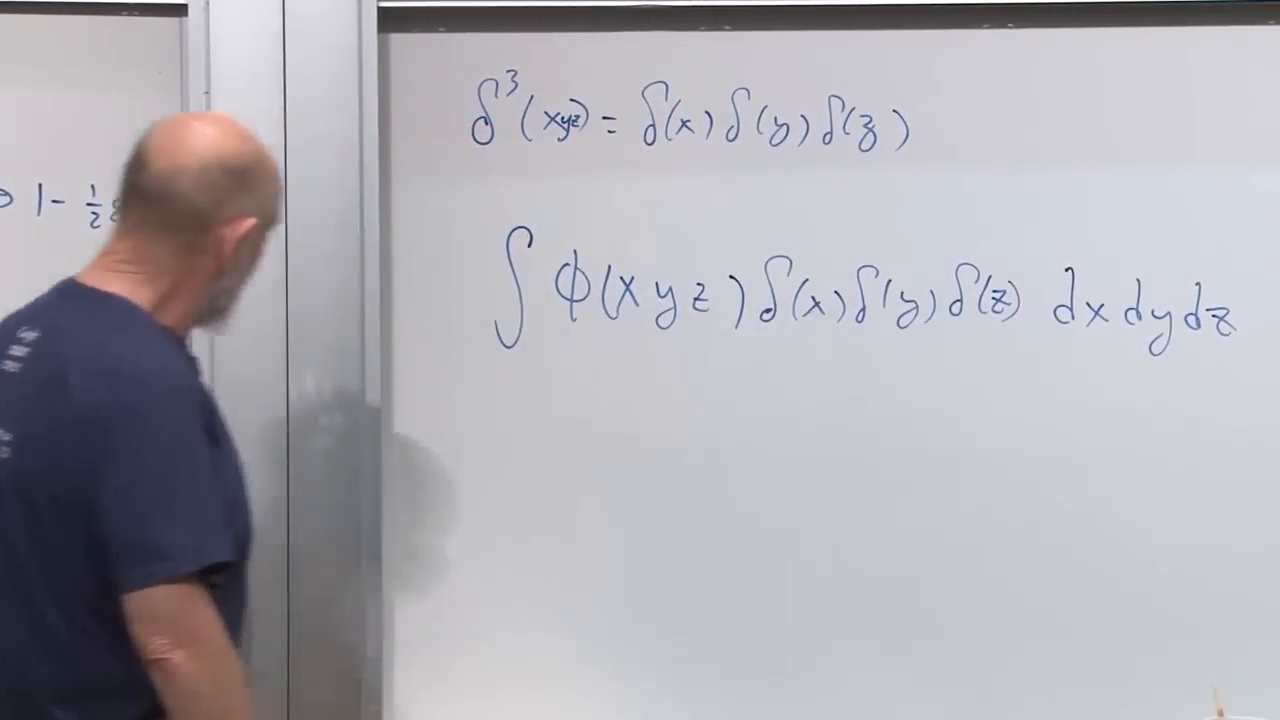
\includegraphics[width=0.90\textwidth]{lecture_05_figure_10.png}
\caption{3つの1次元因子に展開された3次元デルタ関数。}
\lectureframe{00:39:05}
\end{figure}

\eqref{eq:sr5-worldline-interaction}は今や次のように書ける。
\begin{equation}
S_{\mathrm{int}}
=
-g\int d^4x\,
\delta^3(\mathbf{x})\phi(\mathbf{x},t).
\end{equation}
完全な静的源の作用は
\begin{align}
S
=
\int d^4x
\biggl\{
&\frac12(\partial_t\phi)^2
-\frac12|\boldsymbol{\nabla}\phi|^2
\nonumber\\
&-g\delta^3(\mathbf{x})\phi
\biggr\}.
\label{eq:sr5-combined-action}
\end{align}

\begin{classroomqa}
\audiencequestion{相互作用を時空の作用に挿入したとき、マイナス符号が失われなかったか。}
\lecturerresponse{世界線ラグランジアンには\(-g\phi\)が含まれるので、時空の密度には\(-g\delta^3(\mathbf{x})\phi\)が含まれなければならない。その符号を保つことで、場の方程式の源項が確定する。\lecturetimestamp{00:41:24}}
\end{classroomqa}

\begin{figure}[htbp]
\centering
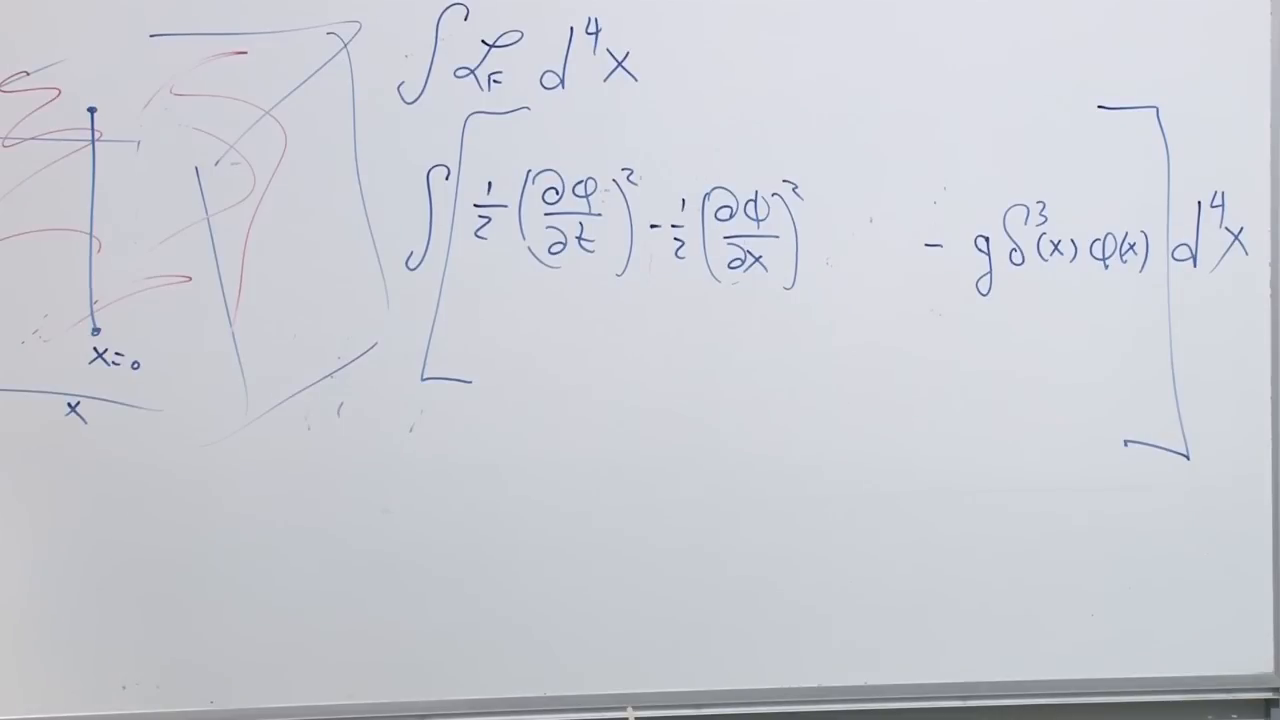
\includegraphics[width=0.90\textwidth]{lecture_05_figure_11.png}
\caption{自由スカラー密度と局在した相互作用が一つの時空の作用に組み立てられた。}
\lectureframe{00:42:05}
\end{figure}

\subsection{源のある場の方程式}

\eqref{eq:sr5-combined-action}を\(\phi\)について変分すると
\begin{equation}
\boxed{
\partial_t^2\phi-\nabla^2\phi
=
-g\delta^3(\mathbf{x})
}.
\label{eq:sr5-sourced-wave}
\end{equation}
原点から離れたところでは、これは自由波動方程式である。原点では、デルタ関数が粒子を局在した源として示す。

\begin{figure}[htbp]
\centering
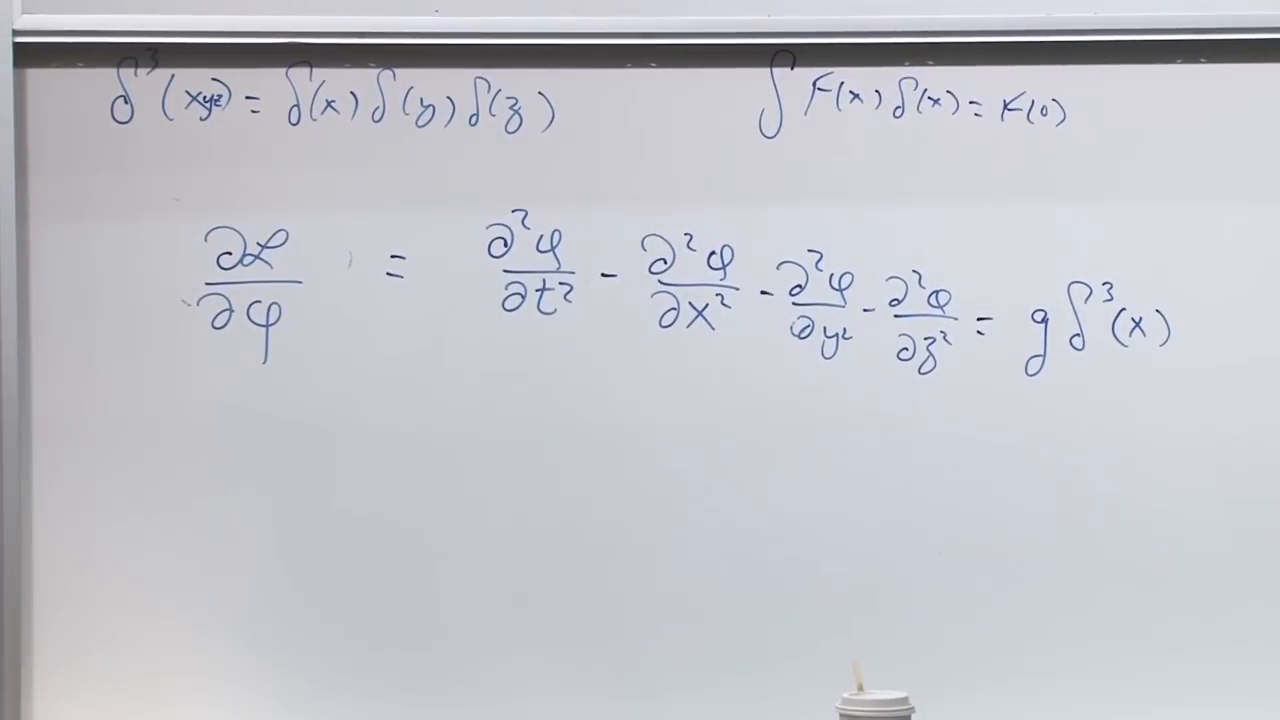
\includegraphics[width=0.90\textwidth]{lecture_05_figure_12.png}
\caption{原点の点源によって駆動される波動演算子。}
\lectureframe{00:45:35}
\end{figure}

静的解では\(\partial_t\phi=0\)であるから、
\begin{equation}
\boxed{
\nabla^2\phi
=
g\delta^3(\mathbf{x})
}.
\label{eq:sr5-poisson}
\end{equation}
これは点源に対するポアソン方程式である。この類推は静電的であり、まだ電磁的ではない。場は依然としてスカラー\(\phi\)であり、電磁四元ポテンシャルではない。

\begin{figure}[htbp]
\centering
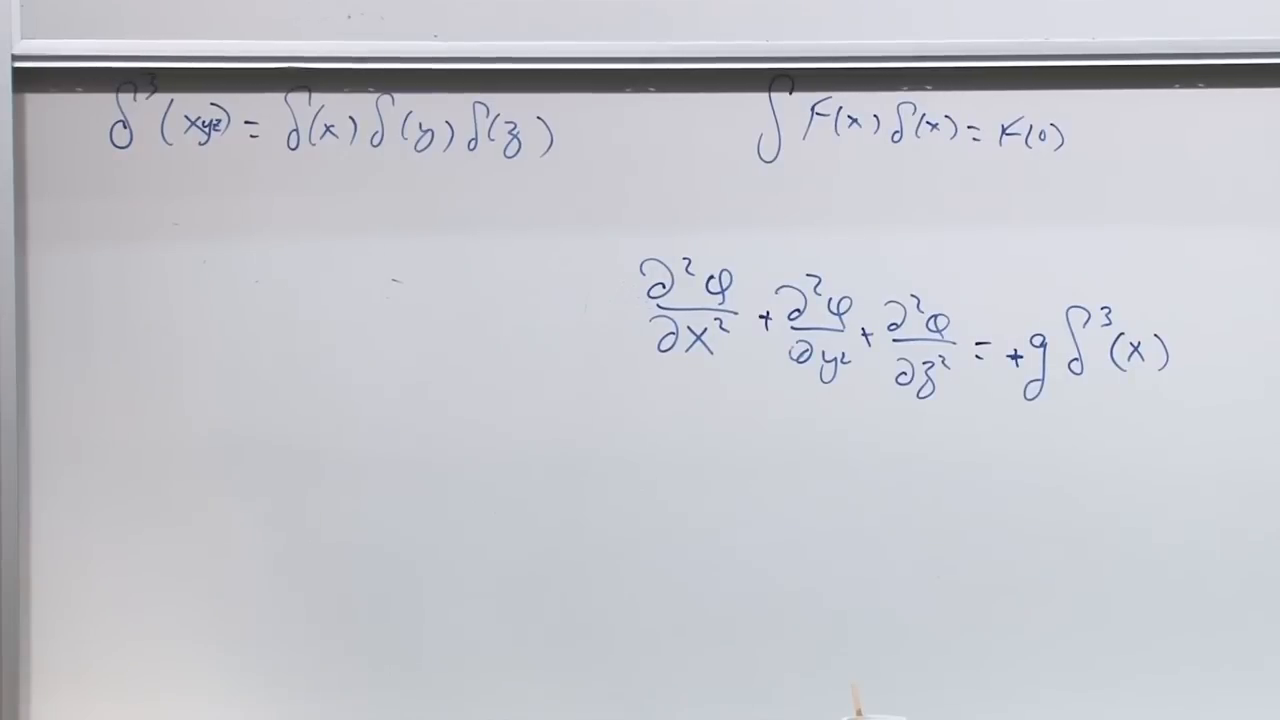
\includegraphics[width=0.90\textwidth]{lecture_05_figure_13.png}
\caption{源のある波動方程式の静的極限であり、ポアソン方程式として認識される。}
\lectureframe{00:47:05}
\end{figure}

相互性が今や明示的である。項\(g\phi\)は粒子にポテンシャルエネルギーを与え、同じ\(g\)が粒子を\(\phi\)の源にする。この二つの効果は独立な仮定ではない。

\subsection{運動する源は放射する}

\(\mathbf{a}\)に固定された粒子は
\(\delta^3(\mathbf{x}-\mathbf{a})\)で表される。その位置が時間とともに変化するなら、源は
\begin{equation}
\delta^3\!\left(\mathbf{x}-\mathbf{a}(t)\right).
\label{eq:sr5-moving-delta}
\end{equation}
となる。時間に依存する右辺は、時間に依存しない場では釣り合いを取れない。\(\partial_t^2\phi\)の項が戻らなければならず、加速または振動する源は場に波を放出しうる。

\begin{figure}[htbp]
\centering
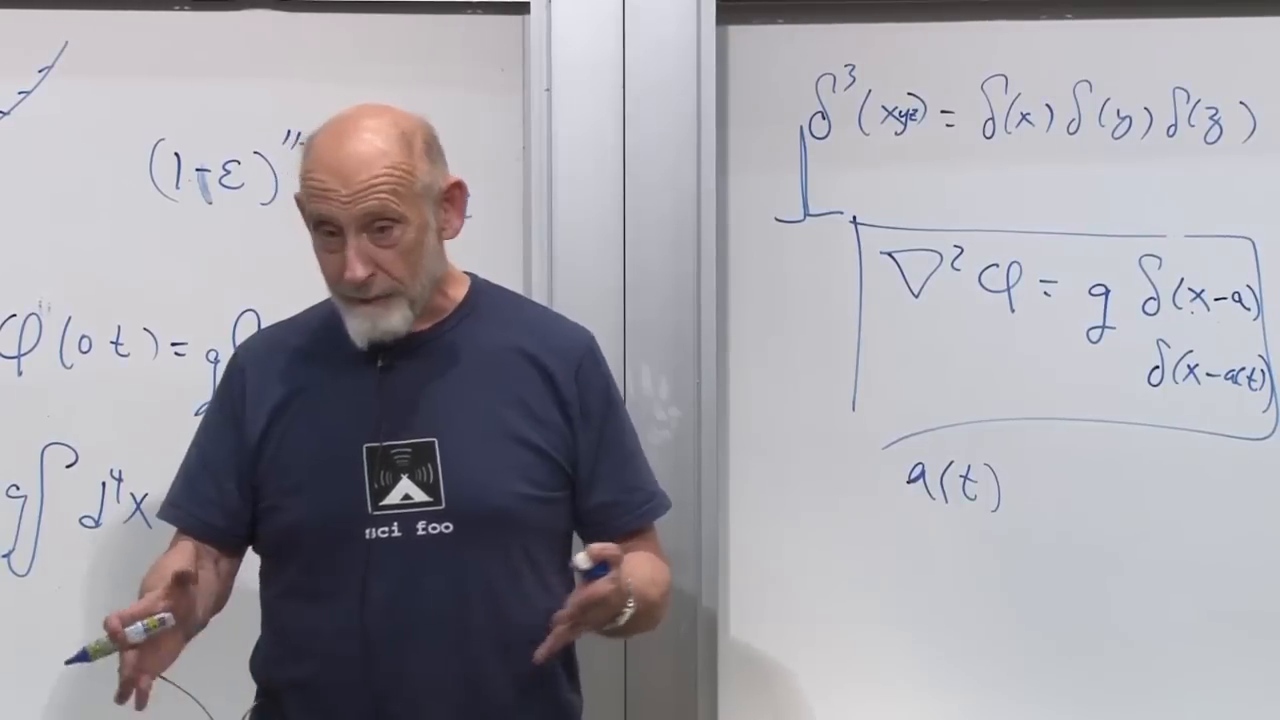
\includegraphics[width=0.90\textwidth]{lecture_05_figure_14.png}
\caption{\(\mathbf{a}(t)\)に移されたデルタ関数源であり、場の方程式を時間依存にする。}
\lectureframe{00:50:30}
\end{figure}

\begin{classroomqa}
\audiencequestion{源を非相対論的に扱うなら、場の方程式のどこに相対性があるのか。}
\lecturerresponse{相対論的な伝播は左辺の時空波動演算子に符号化されている。完全に相対論的な粒子の扱いでは、その固有時間の作用と速度因子が保たれるであろう。ゆっくり動くが時間依存の源でさえ波を駆動しうる。\lecturetimestamp{00:52:14}}
\end{classroomqa}

\begin{classroomqa}
\audiencequestion{\(g\phi\)はどのような単位を持たなければならないか。}
\lecturerresponse{それは粒子の作用において\(mc^2\)の隣に現れるので、エネルギーの単位を持つ。ここで用いられている自然単位の規格化では、\(3+1\)次元のスカラーは質量次元1を持ち、\(g\)は無次元でありうる。次元は時空の次元と場の規格化によって変わる。\lecturetimestamp{00:52:55}}
\end{classroomqa}

\section{四元ベクトル、スカラー、計量}

成分方程式は、より良い記法を正当化するほど長くなってきた。時空座標を
\begin{equation}
x^\mu=(x^0,x^1,x^2,x^3)=(t,x,y,z),
\label{eq:sr5-four-coordinate}
\end{equation}
と書く。ここでギリシャ文字の添字は四つの成分すべてにわたって走る。四成分のリストは自動的に四元ベクトルではない。その成分がローレンツ変換の下で\(x^\mu\)と同様に変換する場合にのみ、それは四元ベクトルである。

\begin{figure}[htbp]
\centering
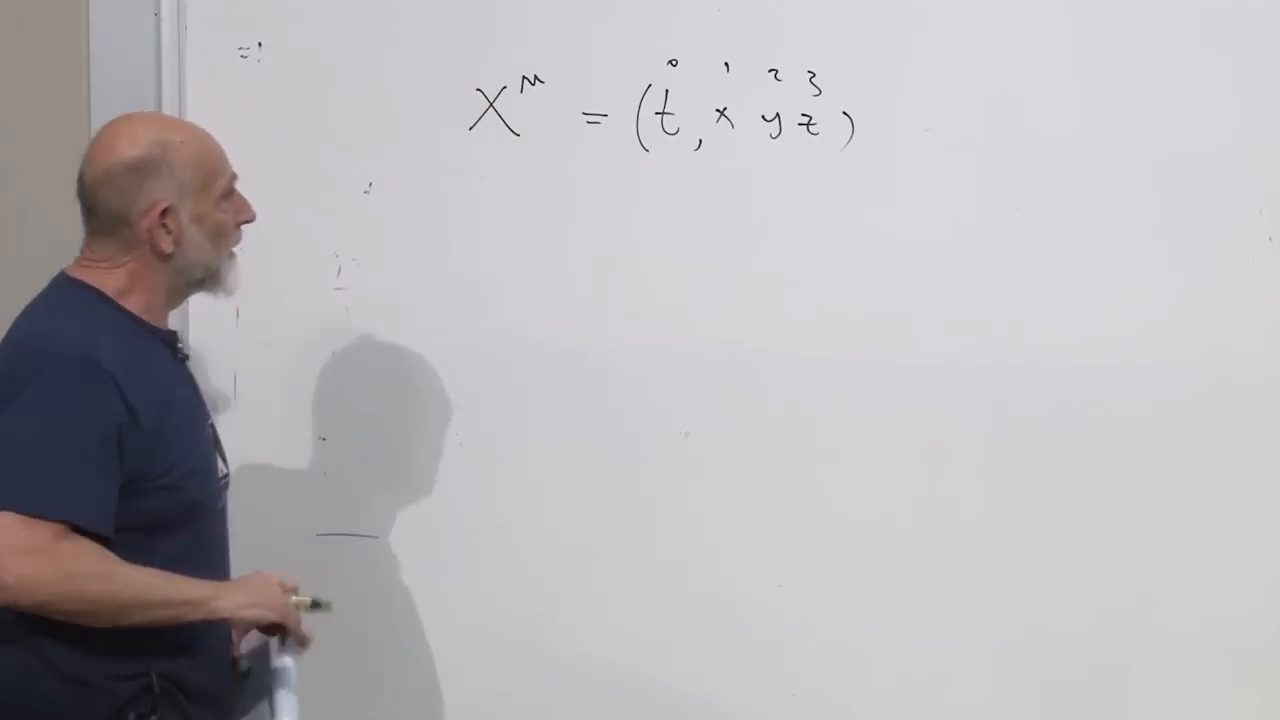
\includegraphics[width=0.90\textwidth]{lecture_05_figure_15.png}
\caption{四つの時空座標を\(x^\mu\)にまとめたもの。}
\lectureframe{00:55:00}
\end{figure}

三つの空間成分が消えるという主張は、ある座標系では成り立ち、別の座標系では成り立たないかもしれない。対照的に、四つの成分すべてが消えるなら、すべてのローレンツ観測者がそのベクトルはゼロであることに同意する。\(dx^\mu\)のような差もまた四元ベクトルである。

不変な固有時間間隔は
\begin{equation}
d\tau^2
=
dt^2-dx^2-dy^2-dz^2.
\label{eq:sr5-proper-time}
\end{equation}
である。それは四つの座標系依存の成分ではなく一つの値を持つので、スカラーである。

\begin{figure}[htbp]
\centering
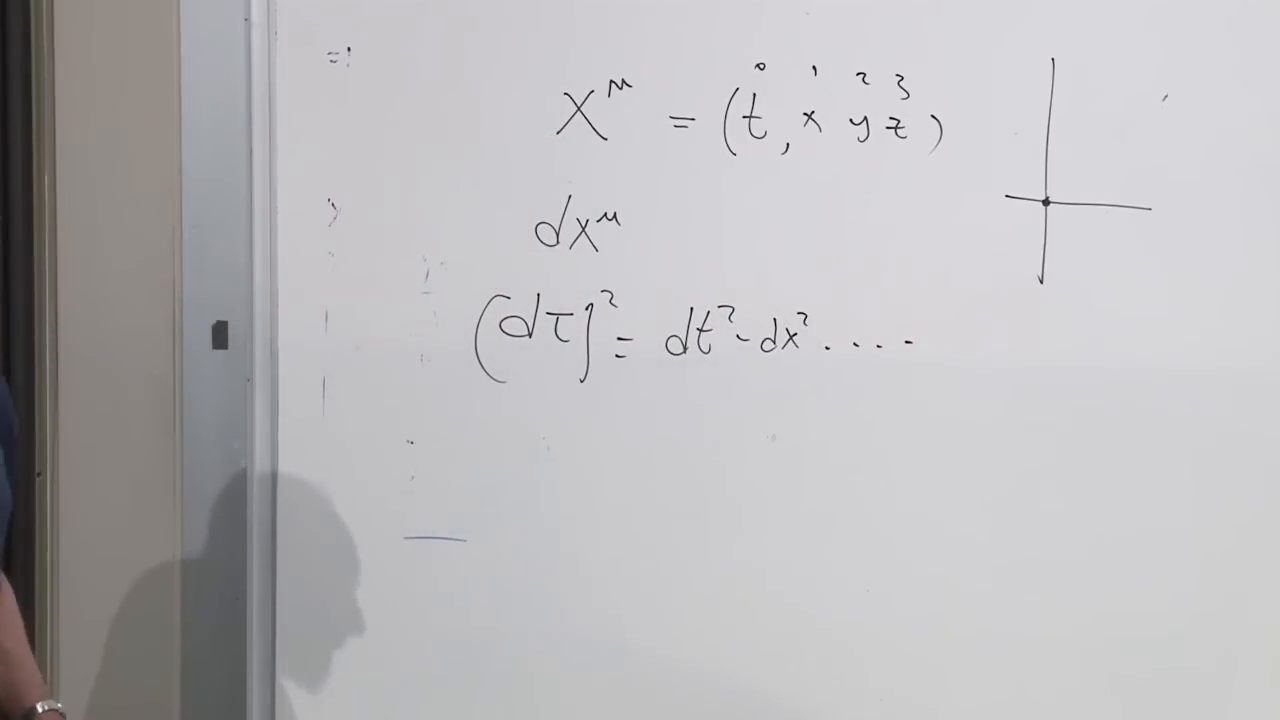
\includegraphics[width=0.90\textwidth]{lecture_05_figure_16.png}
\caption{四元変位と不変な固有時間間隔。}
\lectureframe{00:57:25}
\end{figure}

\subsection{ミンコフスキー計量}

mostly-plusの符号数
\begin{equation}
\eta_{\mu\nu}
=
\operatorname{diag}(-1,1,1,1).
\label{eq:sr5-metric}
\end{equation}
を採用する。代わりのmostly-minusの規約も同様に有効であるが、すべての方程式は一つの規約を一貫して用いなければならない。\eqref{eq:sr5-metric}の下で、
\begin{equation}
dx^\mu dx_\mu
=
-dt^2+dx^2+dy^2+dz^2
=
-d\tau^2.
\end{equation}
全体の符号は不変性を変えない。

\begin{figure}[htbp]
\centering
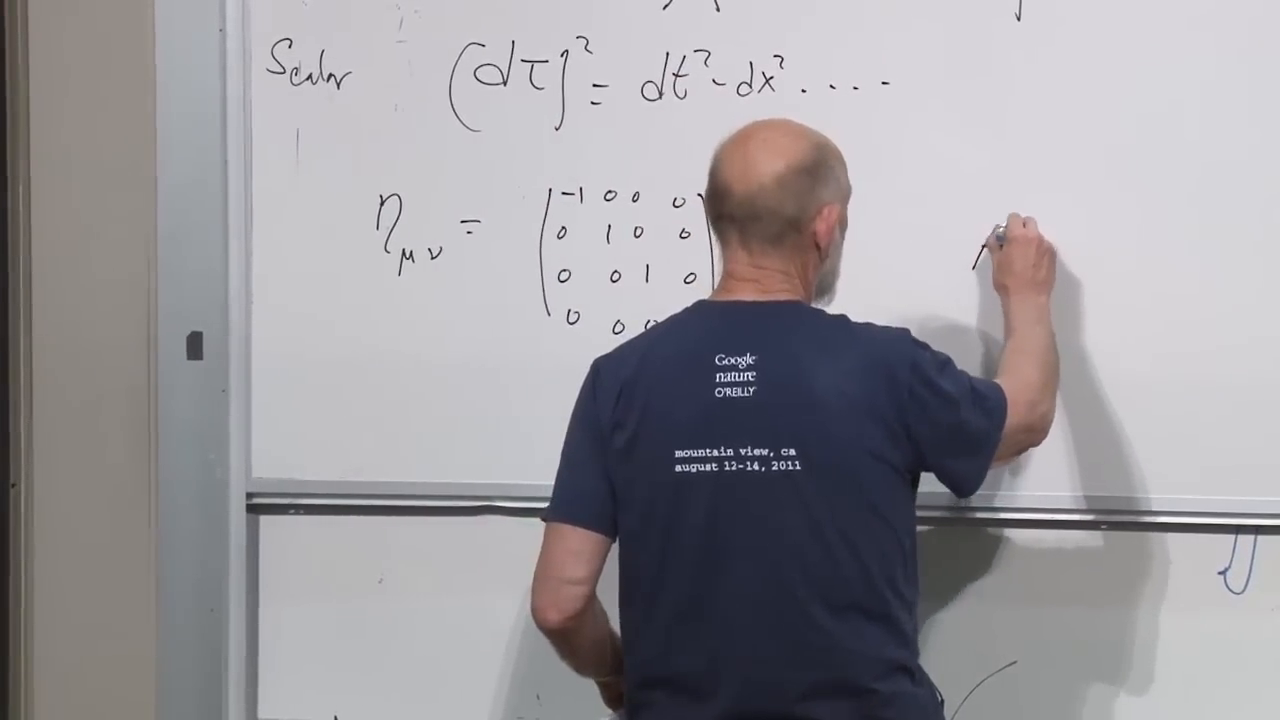
\includegraphics[width=0.90\textwidth]{lecture_05_figure_17.png}
\caption{対角行列として書かれたmostly-plusのミンコフスキー計量。}
\lectureframe{01:00:30}
\end{figure}

計量は添字を下げる。
\begin{equation}
A_\mu=\eta_{\mu\nu}A^\nu.
\label{eq:sr5-lower-index}
\end{equation}
このデカルト計量では、
\begin{equation}
A^\mu=(A^0,A^1,A^2,A^3),
\qquad
A_\mu=(-A^0,A^1,A^2,A^3).
\label{eq:sr5-upper-lower-components}
\end{equation}
同じ計量をもう一度適用すると、\(\eta^{\mu\rho}\eta_{\rho\nu}=\delta^\mu{}_\nu\)であるから添字が上がる。

\begin{figure}[htbp]
\centering
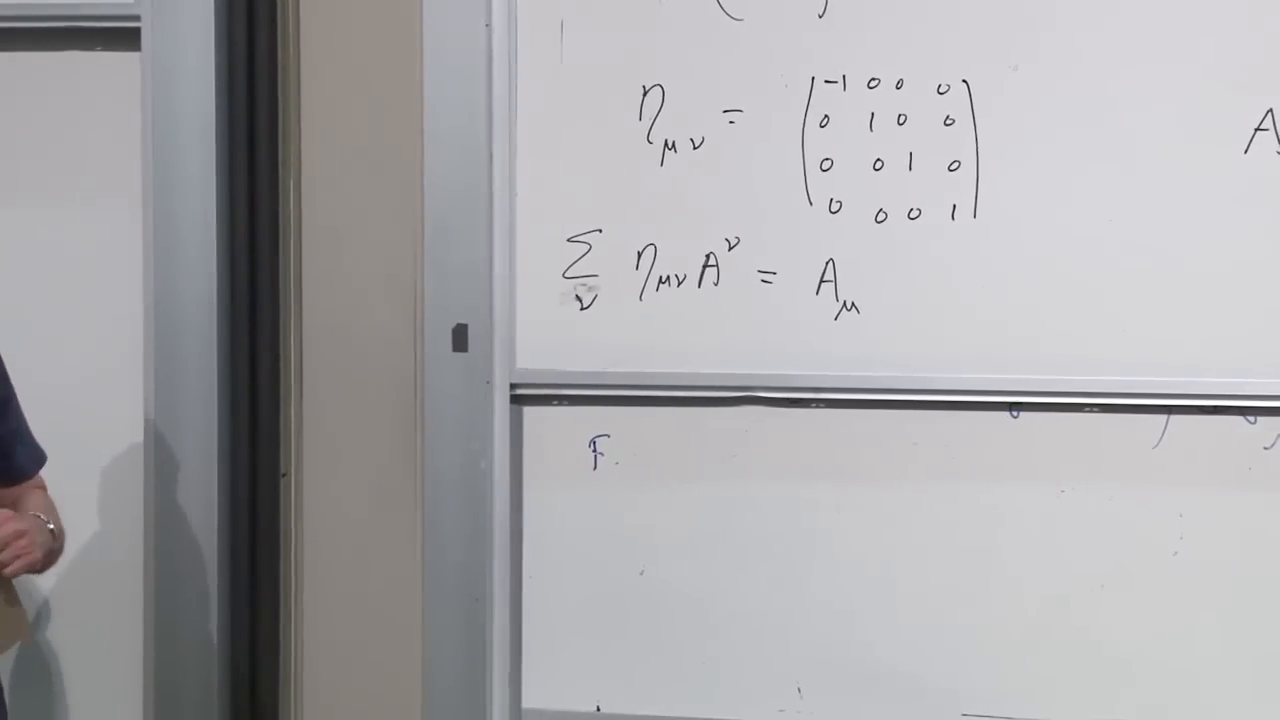
\includegraphics[width=0.90\textwidth]{lecture_05_figure_18.png}
\caption{\(\eta_{\mu\nu}\)による行列積としての添字下げ。}
\lectureframe{01:03:00}
\end{figure}

\begin{classroomqa}
\audiencequestion{ここで通常の行列の積には本当に和が含まれているのか。}
\lecturerresponse{はい。各出力成分は\(\eta\)の一行にベクトル全体を掛けたものであり、列の添字に関する和である。対角な計量のおかげで計算は自明に見えるが、一般の行列ではその和が明示的になる。\lecturetimestamp{01:04:56}}
\end{classroomqa}

\subsection{アインシュタインの縮約と自由添字}

アインシュタインの規約では、添字が上に一度、下に一度現れるたびに和の記号を省略する：
\begin{equation}
\eta_{\mu\nu}A^\nu
\equiv
\sum_{\nu=0}^{3}\eta_{\mu\nu}A^\nu.
\end{equation}
ここで\(\nu\)はダミー添字であり、和をとって消えるので名前を変えてもよい。添字\(\mu\)は自由添字であり、結果の四つの成分にラベルを付ける。一つの単項式の中に同じ添字が二度より多く現れることは通常ない。

伝統的な名称は、上付き添字に対して\emph{反変}、下付き添字に対して\emph{共変}である。この講義では意図的に、より平易な\emph{上付き}と\emph{下付き}という言葉を好んで用いるが、どちらの用語も同じ変換則を指している。

\section{スカラーの縮約と微分}

\subsection{ミンコフスキー内積}

ベクトルをその下付きの形と縮約すると
\begin{equation}
A^\mu A_\mu
=
\eta_{\mu\nu}A^\mu A^\nu
=
-(A^0)^2+(A^1)^2+(A^2)^2+(A^3)^2.
\label{eq:sr5-vector-square}
\end{equation}
となる。余分なマイナス符号を手で挿入してはならない。それはすでに下付きの時間成分から来ている。

\begin{figure}[htbp]
\centering
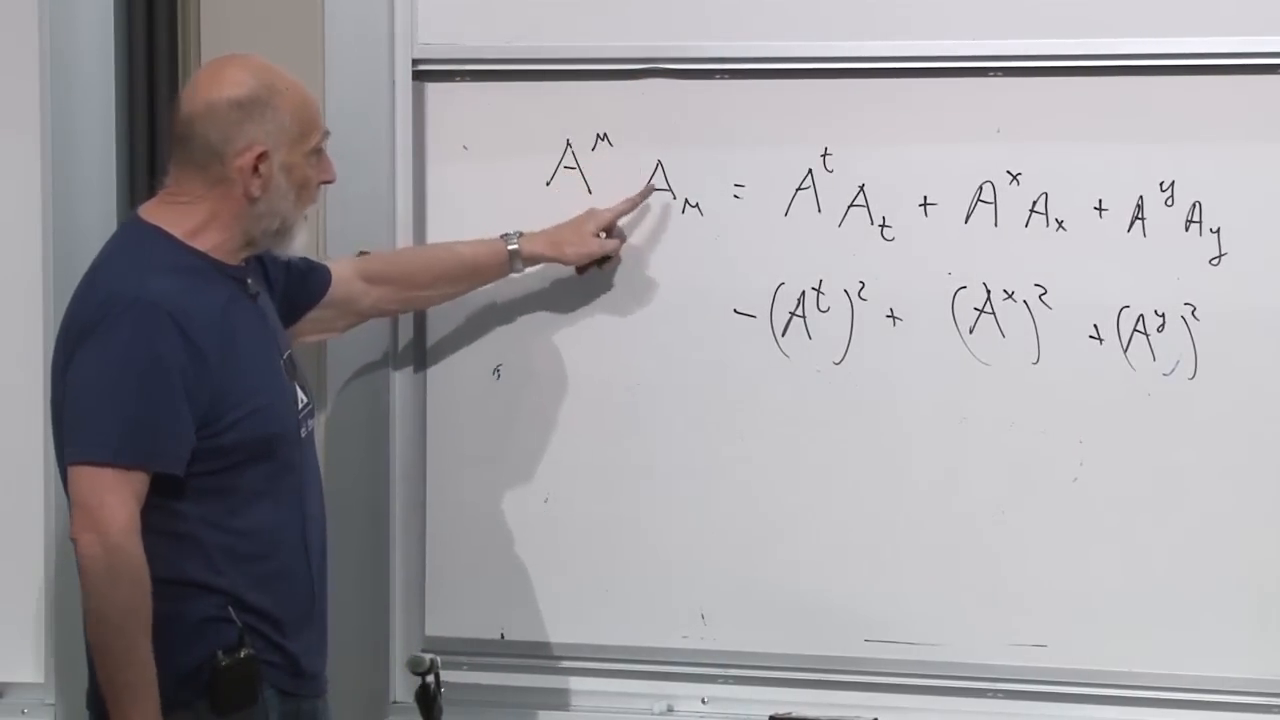
\includegraphics[width=0.90\textwidth]{lecture_05_figure_19.png}
\caption{縮約\(A^\mu A_\mu\)を時間成分と空間成分に展開したもの。}
\lectureframe{01:09:30}
\end{figure}

\begin{classroomqa}
\audiencequestion{下付き添字のベクトルは列ではなく行として描くべきなのか。}
\lecturerresponse{初等的な行列表記では行として表してもよいが、添字記法はその選択を要求しない。その定義的な特徴は、どのように変換し、上付き添字のベクトルとどのように縮約するかにある。\lecturetimestamp{01:10:26}}
\end{classroomqa}

\begin{classroomqa}
\audiencequestion{ギリシャ文字の添字は常に四つの成分すべてを指すのか。}
\lecturerresponse{この記法では、はい。\(\mu,\nu\)のようなギリシャ文字の添字は時空全体を走り、\(i,j\)のようなラテン文字の添字は通常、三つの空間成分のみを走る。\lecturetimestamp{01:12:23}}
\end{classroomqa}

同じ構成は二つの異なる四元ベクトルに対しても成り立つ：
\begin{equation}
A^\mu B_\mu
\end{equation}
はスカラーである。一つの手早い証明は偏極恒等式を用いる。
\((A+B)^2\)と\((A-B)^2\)はどちらもスカラーであるから、
\begin{equation}
(A+B)^2-(A-B)^2=4A^\mu B_\mu
\end{equation}
もまたスカラーである。これは通常のドット積のミンコフスキー版である。

\begin{classroomqa}
\audiencequestion{\(A^\mu B_\mu\)は通常のドット積に類似しているのか。}
\lecturerresponse{そのとおりである。ただしミンコフスキー計量が時間成分と空間成分の間の相対的な符号を与える。\lecturetimestamp{01:15:44}}
\end{classroomqa}

\subsection{勾配は余ベクトルである}

\(\phi(x)\)をスカラー場とし、\(x\)は今や四つの時空座標すべてを表すものとする。隣り合う事象の間で、
\begin{equation}
d\phi
=
\frac{\partial\phi}{\partial x^\mu}dx^\mu
=
\partial_\mu\phi\,dx^\mu.
\label{eq:sr5-dphi}
\end{equation}
左辺はスカラーであり、\(dx^\mu\)は四元ベクトルである。したがって係数
\begin{equation}
\partial_\mu\phi
=
\left(
\partial_t\phi,
\partial_x\phi,
\partial_y\phi,
\partial_z\phi
\right)
\label{eq:sr5-gradient-lower}
\end{equation}
は余ベクトルとして変換しなければならない。その添字を上げると
\begin{equation}
\partial^\mu\phi
=
\left(
-\partial_t\phi,
\partial_x\phi,
\partial_y\phi,
\partial_z\phi
\right).
\label{eq:sr5-gradient-upper}
\end{equation}
となる。

\begin{figure}[htbp]
\centering
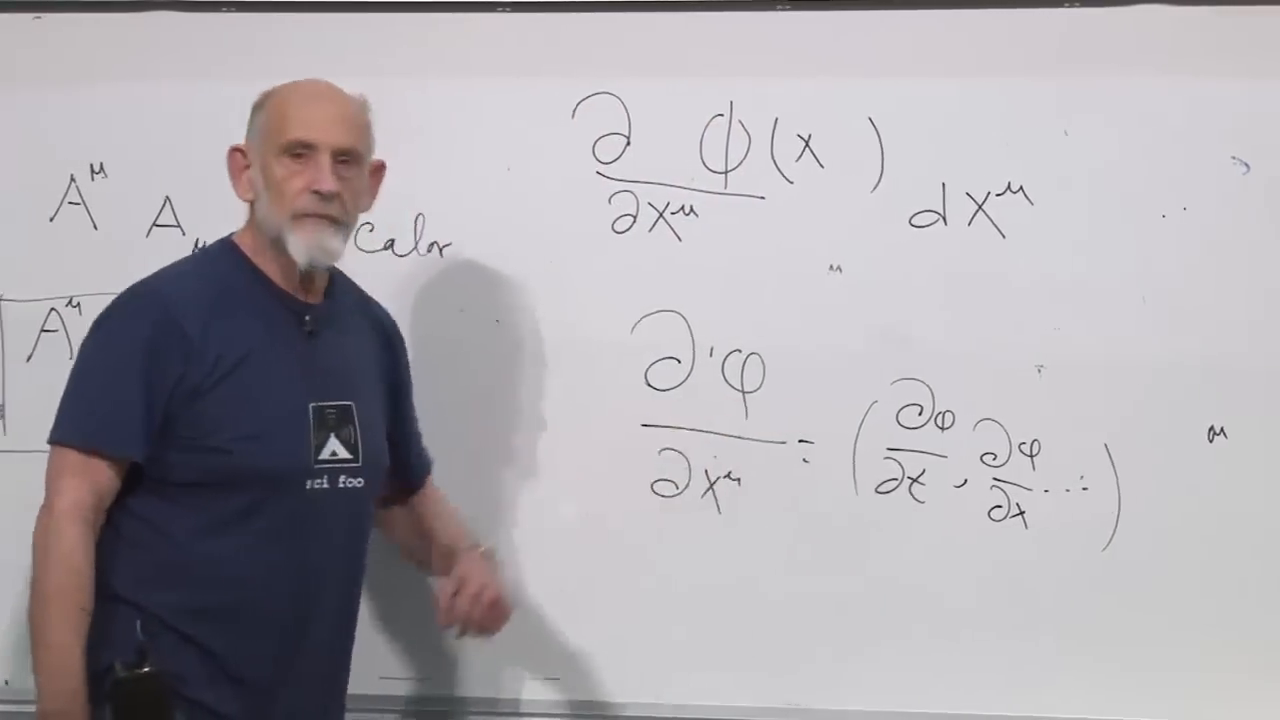
\includegraphics[width=0.90\textwidth]{lecture_05_figure_20.png}
\caption{微分\(d\phi=\partial_\mu\phi\,dx^\mu\)。これからスカラー勾配の余ベクトルとしての性質が従う。}
\lectureframe{01:20:00}
\end{figure}

\begin{classroomqa}
\audiencequestion{\(x^\mu\)の上付き添字は、分母\(\partial/\partial x^\mu\)に現れると下付き添字になるのか。}
\lecturerresponse{はい。座標微分\(dx^\mu\)は反変的に変換するので、その双対な微分\(\partial_\mu=\partial/\partial x^\mu\)は共変的に変換する。それによって\(d\phi=\partial_\mu\phi\,dx^\mu\)がスカラーになるのである。\lecturetimestamp{01:20:00}}
\end{classroomqa}

\subsection{不変なスカラー場の密度}

二つの微分ベクトルを縮約すると
\begin{align}
\partial_\mu\phi\,\partial^\mu\phi
&=
-(\partial_t\phi)^2
+(\partial_x\phi)^2
+(\partial_y\phi)^2
+(\partial_z\phi)^2.
\end{align}
となる。したがって自由スカラー密度は
\begin{equation}
\boxed{
\mathcal L_0
=
-\frac12
\partial_\mu\phi\,\partial^\mu\phi
}.
\label{eq:sr5-compact-density}
\end{equation}
と簡潔に書ける。これは\eqref{eq:sr5-free-field-action}の成分密度と同一である。

\begin{figure}[htbp]
\centering
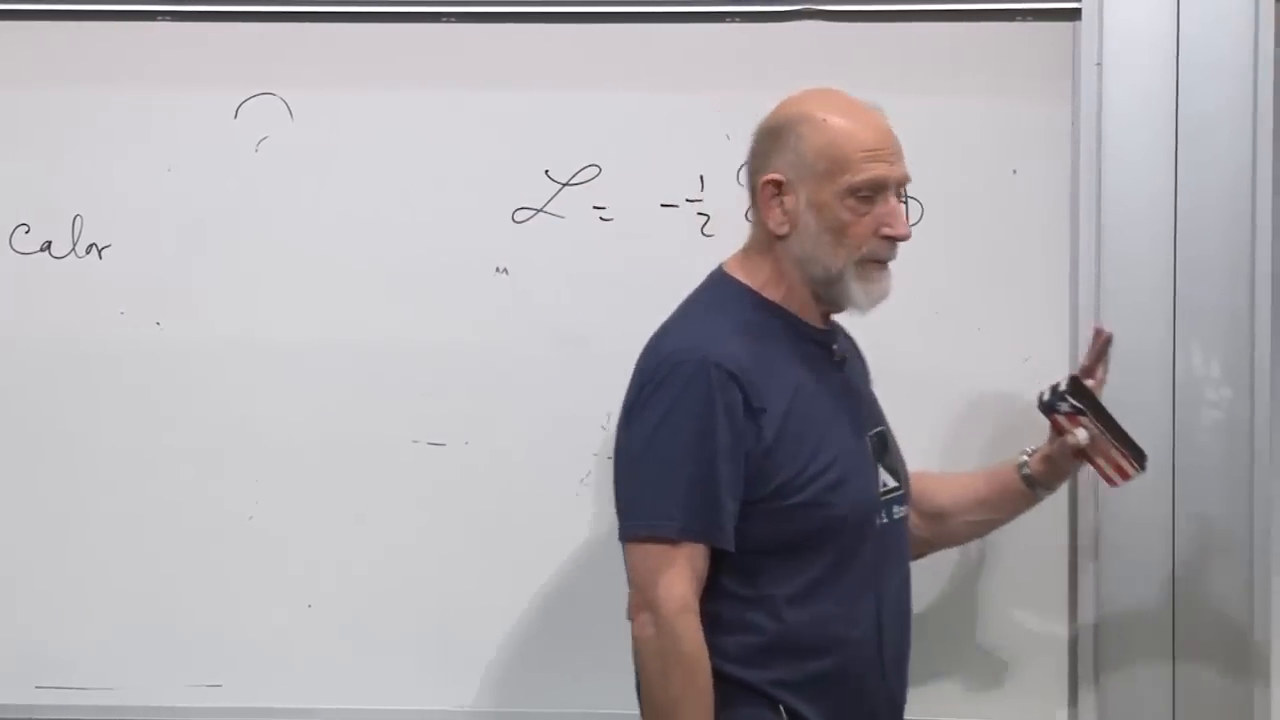
\includegraphics[width=0.90\textwidth]{lecture_05_figure_21.png}
\caption{スカラー場の運動項密度を一つの縮約された表式にまとめたもの。}
\lectureframe{01:25:10}
\end{figure}

\begin{classroomqa}
\audiencequestion{この縮約された一階微分の表式はラプラシアンなのか。}
\lecturerresponse{いいえ。ラプラシアンは二階の空間微分を含む。この表式はラグランジアン密度であり、一階微分の積から作られている。\lecturetimestamp{01:24:38}}
\end{classroomqa}

物理的な事象におけるスカラー密度の値は座標系に依存しない。固有ローレンツ変換もまた行列式の大きさが1であるから、測度\(d^4x\)は不変である。したがって、
\begin{equation}
S=\int d^4x\,\mathcal L
\end{equation}
は不変である。座標系に依存しない作用は、すべての慣性系で同じ形のオイラー--ラグランジュ方程式を与える。

\section{ガリレイ極限}

\begin{classroomqa}
\audiencequestion{ニュートン力学のラグランジアンも相対性原理を尊重することが要求されていたのであろうか。}
\lecturerresponse{はい、ただしそれは以前には強調されていなかった。ニュートンの方程式は、ローレンツ変換の\(c\to\infty\)極限であるガリレイ変換の下で不変である。その極限で消えるのは同時性の相対性である。\lecturetimestamp{01:27:16}}
\end{classroomqa}

その極限を見るために、\(x\)に沿ったブーストにおいて\(c\)を復元すると、
\begin{equation}
x'
=
\frac{x-vt}{\sqrt{1-v^2/c^2}},
\qquad
t'
=
\frac{t-vx/c^2}{\sqrt{1-v^2/c^2}}.
\label{eq:sr5-lorentz-c}
\end{equation}
\(c\to\infty\)とすると
\begin{equation}
\boxed{
x'=x-vt,
\qquad
t'=t
}.
\label{eq:sr5-galilean}
\end{equation}
が得られる。これらはガリレイ変換である。ニュートン力学は、法則があらゆる慣性系で同じ形をとるという相対性原理を保持しているが、同時にすべての観測者に共有される絶対時間も仮定している。

\begin{figure}[htbp]
\centering
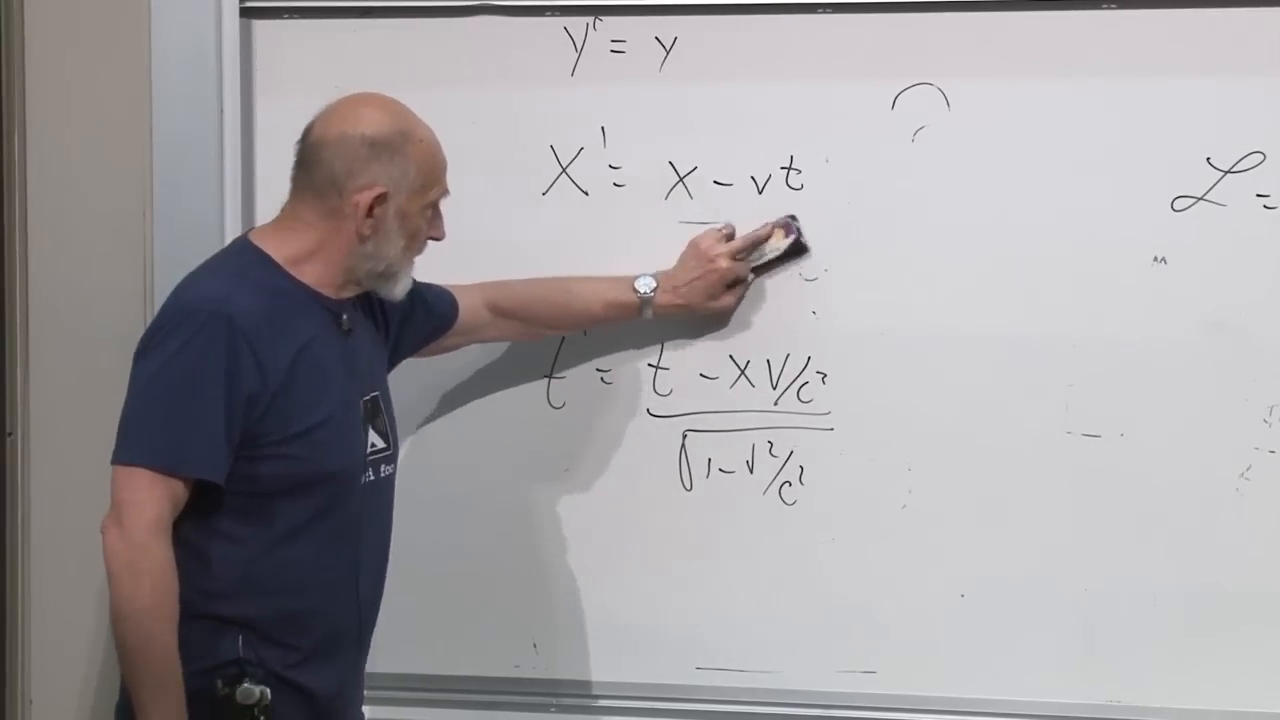
\includegraphics[width=0.90\textwidth]{lecture_05_figure_22.png}
\caption{\(c\to\infty\)をとる前のローレンツブーストであり、ガリレイの規則\(x'=x-vt\)および\(t'=t\)を残す。}
\lectureframe{01:29:40}
\end{figure}

\begin{classroomqa}
\audiencequestion{上付き添字と下付き添字のベクトルは符号の変化だけによって異なって変換されるのであろうか。}
\lecturerresponse{ここで用いられている固定されたデカルト計量では、すでに知られているベクトルを下げることはその時間成分の符号を変えるだけである。それにもかかわらず、それらのローレンツ変換則は単なる恣意的な符号の規約ではなく双対な法則であり、一方を他方に変換するのは計量である。\lecturetimestamp{01:31:19}}
\end{classroomqa}

\begin{classroomqa}
\audiencequestion{座標の一見普通の関数はすべてスカラーなのであろうか。}
\lecturerresponse{いいえ。各座標点で1つの数であるだけでは十分ではない。その数は、あらゆる系において同じ事象で同じ物理的値を表していなければならない。エネルギー密度は反例である。箱をブーストすると測定されるエネルギーと測定される体積の両方が変化するので、観測者は同じ密度を割り当てない。\lecturetimestamp{01:33:23}}
\end{classroomqa}

四元速度の単一の成分がもう一つの例を与える。完全な四元速度はベクトルであるが、その時間成分はブーストの下で変化し、それ自体はスカラーではない。

\section{クライン--ゴルドン場}

\subsection{調和振動子の場の類似物}

スカラー密度に戻り、最も単純な二次ポテンシャルを加える。
\begin{equation}
\boxed{
\mathcal L
=
\frac12
\left[
(\partial_t\phi)^2
-|\boldsymbol{\nabla}\phi|^2
-\mu^2\phi^2
\right]
}.
\label{eq:sr5-kg-density}
\end{equation}
これは
\begin{equation}
L_{\mathrm{osc}}
=
\frac12\dot q^2-\frac12\mu^2q^2.
\end{equation}
の場の理論における類似物である。各空間点は局所的に振動子のように振る舞い、一方で勾配項は隣接する点を結合する。

\begin{figure}[htbp]
\centering
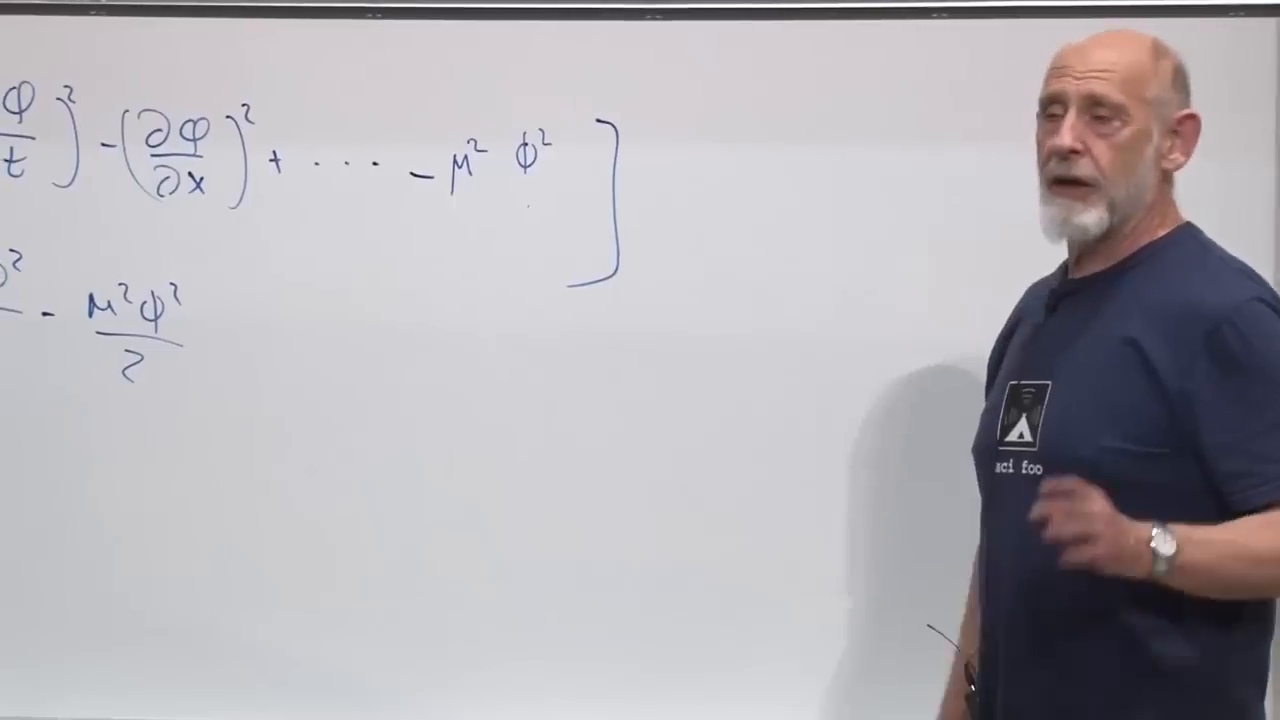
\includegraphics[width=0.90\textwidth]{lecture_05_figure_23.png}
\caption{二次スカラー場の密度とその調和振動子の原型。}
\lectureframe{01:38:20}
\end{figure}

場のオイラー--ラグランジュ方程式は
\begin{equation}
\partial_\mu
\left[
\frac{\partial\mathcal L}
{\partial(\partial_\mu\phi)}
\right]
-
\frac{\partial\mathcal L}{\partial\phi}
=0.
\label{eq:sr5-field-el}
\end{equation}
であり、これを\eqref{eq:sr5-kg-density}に適用すると
\begin{equation}
\boxed{
\partial_t^2\phi-\nabla^2\phi+\mu^2\phi=0
}.
\label{eq:sr5-kg}
\end{equation}
が得られる。これはクライン--ゴルドン方程式である。mostly-plusの規約と\(\Box=\partial_\mu\partial^\mu=-\partial_t^2+\nabla^2\)を用いると、同じ方程式は
\((\Box-\mu^2)\phi=0\)
となる。

\begin{figure}[htbp]
\centering
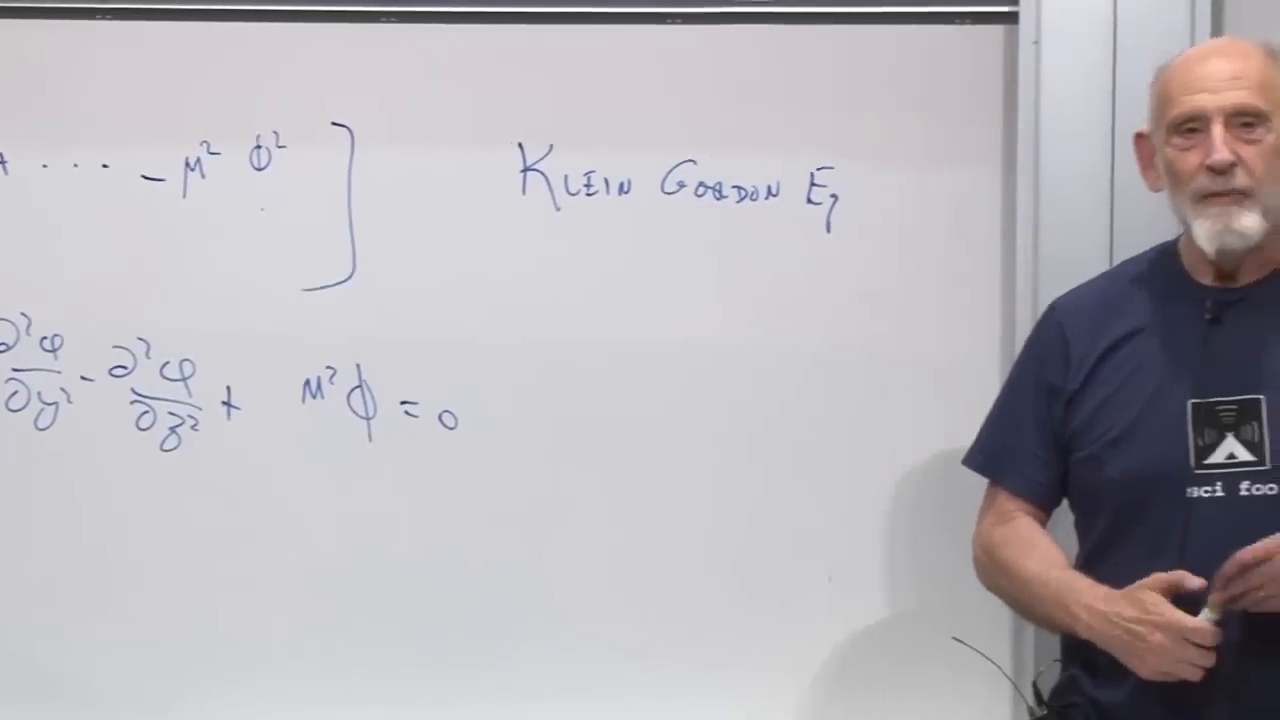
\includegraphics[width=0.90\textwidth]{lecture_05_figure_24.png}
\caption{クライン--ゴルドン方程式が、それが従う密度の下に完成された。}
\lectureframe{01:40:00}
\end{figure}

歴史的には、この方程式は相対論的な単一粒子波動方程式として最初に探究された。その解釈は、特に正の確率密度に関して困難に遭遇した。その本来の現代的設定は相対論的場の理論であり、そこでは自由スカラー場および相互作用するスカラー場の自由極限を支配する。

\subsection{平面波モード}

\eqref{eq:sr5-kg}は定数係数をもつ線形であるから、平面波
\begin{equation}
\phi(x)
=
\exp\!\left[
-i\omega t+i\mathbf{k}\cdot\mathbf{x}
\right].
\label{eq:sr5-plane-wave}
\end{equation}
を求める。
\begin{equation}
k_\mu=(-\omega,k_x,k_y,k_z),
\end{equation}
とすると、指数は\(ik_\mu x^\mu\)である。

\begin{figure}[htbp]
\centering
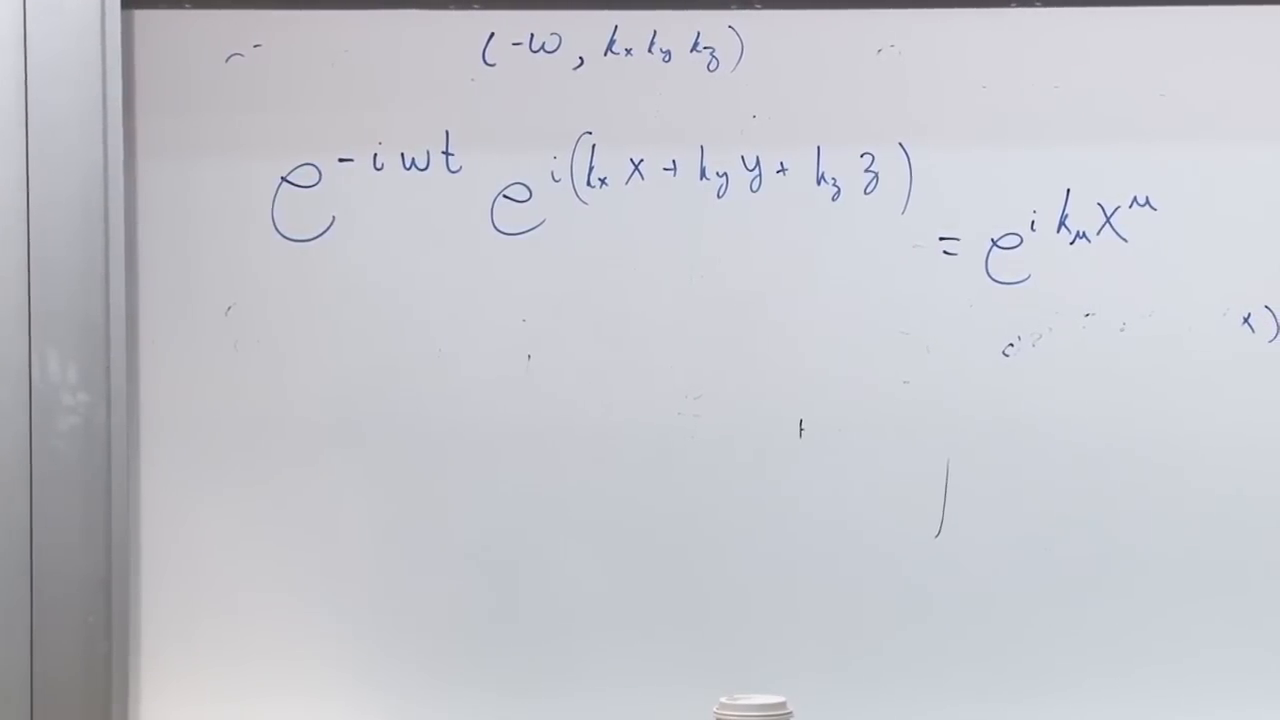
\includegraphics[width=0.90\textwidth]{lecture_05_figure_25.png}
\caption{成分で書かれ、また\(e^{ik_\mu x^\mu}\)として書かれた平面波の仮定。}
\lectureframe{01:44:00}
\end{figure}

微分すると
\begin{equation}
\partial_t^2\phi=-\omega^2\phi,
\qquad
\nabla^2\phi=-|\mathbf{k}|^2\phi.
\end{equation}
が得られる。\eqref{eq:sr5-kg}に代入すると
\begin{equation}
\left(
-\omega^2+|\mathbf{k}|^2+\mu^2
\right)\phi=0.
\end{equation}
が得られる。したがって非零のモードには
\begin{equation}
\boxed{
\omega^2=|\mathbf{k}|^2+\mu^2
},
\qquad
\omega=\pm\sqrt{|\mathbf{k}|^2+\mu^2}.
\label{eq:sr5-dispersion}
\end{equation}
が必要である。

\begin{figure}[htbp]
\centering
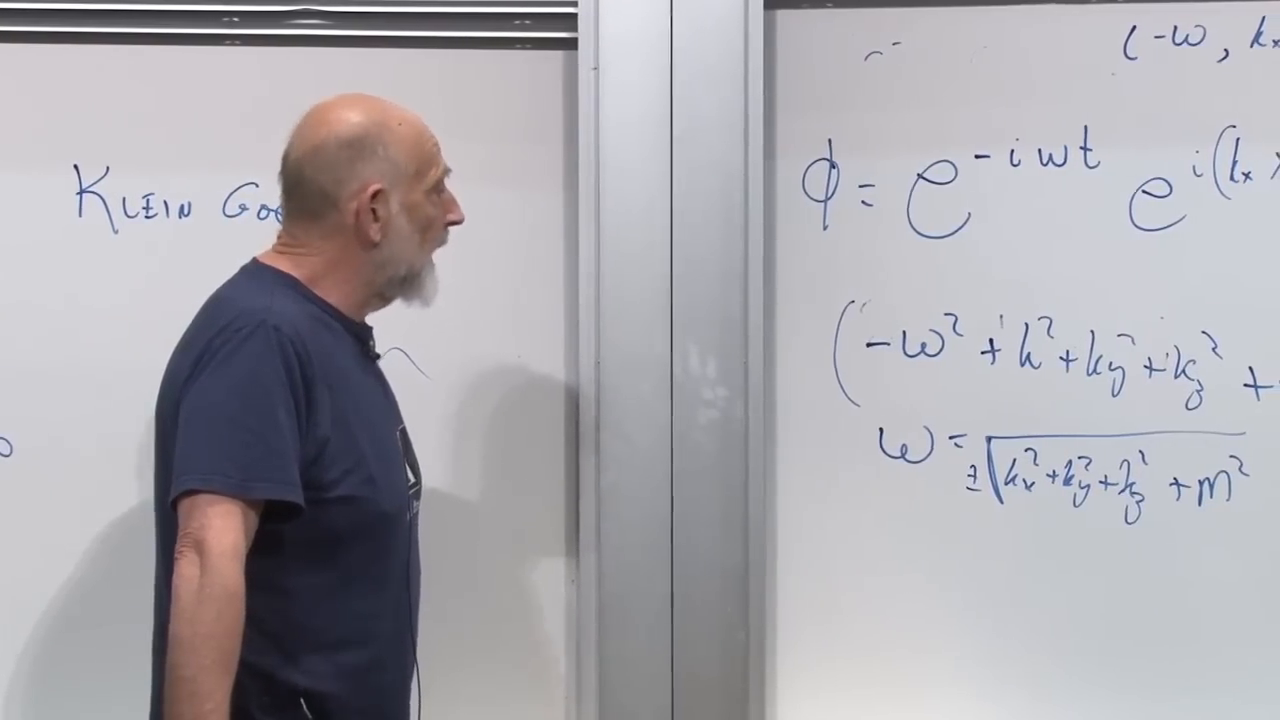
\includegraphics[width=0.90\textwidth]{lecture_05_figure_26.png}
\caption{平面波の代入と、その結果得られる相対論的分散関係。}
\lectureframe{01:47:00}
\end{figure}

自然単位では、\(\mu\)は質量の役割を果たす。量子励起について定数を復元すると、
\begin{equation}
E=\hbar\omega,
\qquad
\mathbf{p}=\hbar\mathbf{k},
\qquad
\mu=\frac{mc}{\hbar},
\end{equation}
により\eqref{eq:sr5-dispersion}は
\begin{equation}
E^2=p^2c^2+m^2c^4.
\end{equation}
となる。正振動数分枝と負振動数分枝はどちらも古典解空間の一部である。一般解はこれらのモードの重ね合わせである。

\begin{classroomqa}
\audiencequestion{クライン--ゴルドン方程式はどこから来たのか。}
\lecturerresponse{それは二次のローレンツスカラー密度から、場のオイラー--ラグランジュ方程式を通じて直接に来る。この例が選ばれたのは、この単純な二次密度が線形な場の方程式を生み出すからである。\lecturetimestamp{01:47:59}}
\end{classroomqa}

\begin{classroomqa}
\audiencequestion{自然界では何がクライン--ゴルドン方程式に従うのか。}
\lecturerresponse{自由な古典スカラー場が従う。ヒッグス場の揺らぎはスカラーであり、自由近似ではクライン--ゴルドン形に帰着するが、実際のヒッグス場は相互作用とゲージ結合ももつ。\lecturetimestamp{01:50:41}}
\end{classroomqa}

\section{質量シフトとしてのスカラー背景}

ここで粒子作用が再び視野に入ってくる：
\begin{equation}
S_{\mathrm p}
=
-\int d\tau\,
\bigl[m+g\phi(x)\bigr].
\label{eq:sr5-final-particle-action}
\end{equation}
\(\phi\) が一定の背景値 \(\phi_0\) をもつなら、粒子はあたかもその質量が
\begin{equation}
\boxed{
m_{\mathrm{eff}}=m+g\phi_0
}.
\label{eq:sr5-effective-mass}
\end{equation}
であるかのように運動する。裸の項 \(m\) が消えるなら、スカラー背景が固有時間に掛かる係数の全体を供給しうる。

\begin{figure}[htbp]
\centering
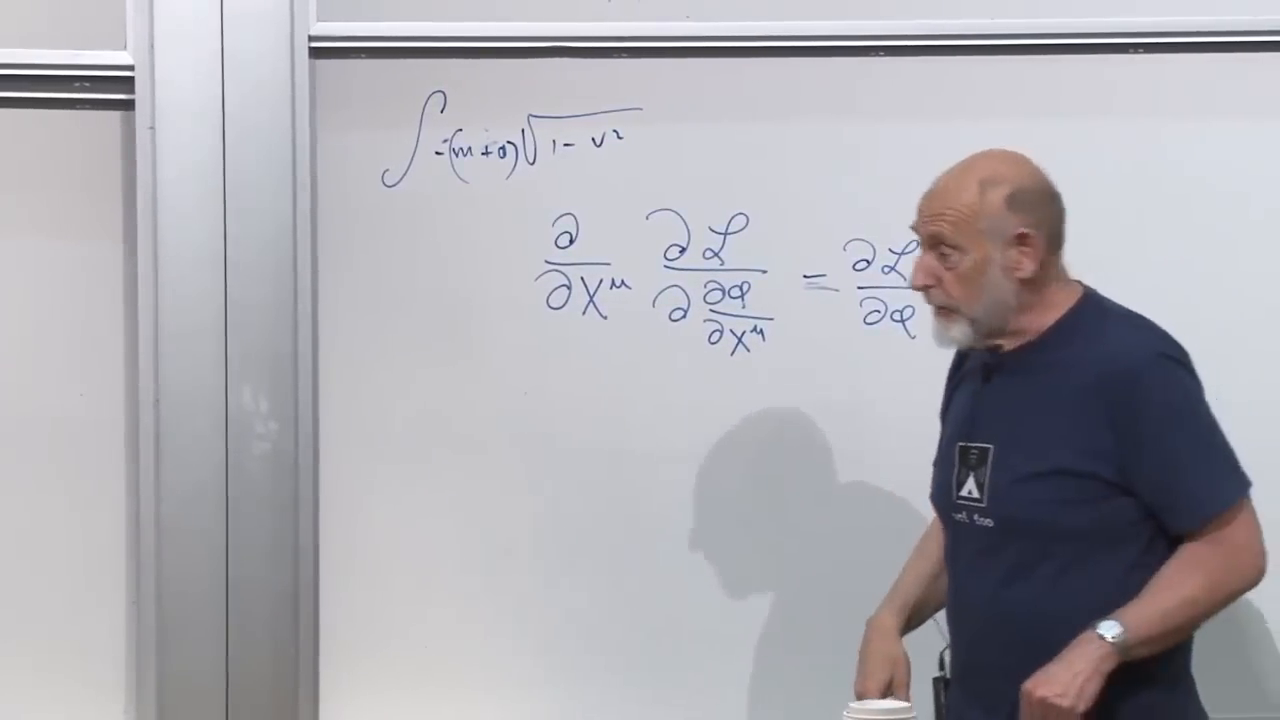
\includegraphics[width=0.90\textwidth]{lecture_05_figure_27.png}
\caption{上記の場に依存する粒子作用は、コンパクトな場のオイラー--ラグランジュ方程式の上にあり、講義の両側面を結び合わせる。}
\lectureframe{01:51:30}
\end{figure}

これはヒッグス質量生成の意図的に単純化された模型である。標準模型では、フェルミオン質量はヒッグス真空期待値への湯川結合から生じ、模式的には \(m_f\propto y_f v\) であり、一方 \(W\) と \(Z\) の質量はゲージ共変なヒッグス運動項を通じて生じる。この玩具的な世界線結合は中心的な考え方--非零のスカラー背景が慣性質量を変える--を捉えており、完全な電弱理論を再現するものではない。先に確立された相互性は依然として有効である：同じ相互作用を場について変分すれば、粒子は源となる。場は粒子に作用し、粒子は場に作用し返す。

\subsection{複素指数関数が有用である理由}

場は物理的に複素である必要はない。オイラーの公式より
\begin{equation}
e^{i(\omega t-\mathbf{k}\cdot\mathbf{x})}
=
\cos(\omega t-\mathbf{k}\cdot\mathbf{x})
+i\sin(\omega t-\mathbf{k}\cdot\mathbf{x}).
\end{equation}
方程式は実かつ線形であるから、実部と虚部はそれぞれ独立に実解である。それらは1周期の4分の1だけずれた波であり、任意の実線形結合もまた解である。

\begin{classroomqa}
\audiencequestion{実部を取るとき、虚部は何らかの形でゼロに加わるのか。}
\lecturerresponse{いいえ。複素指数関数は2つの独立な実解、余弦と正弦をまとめたものである。どちらの部分を保持してもよく、実の組み合わせを作ってもよい。指数関数が用いられるのは、微分が掛け算になるからである。\lecturetimestamp{01:53:29}}
\end{classroomqa}

\begin{figure}[htbp]
\centering
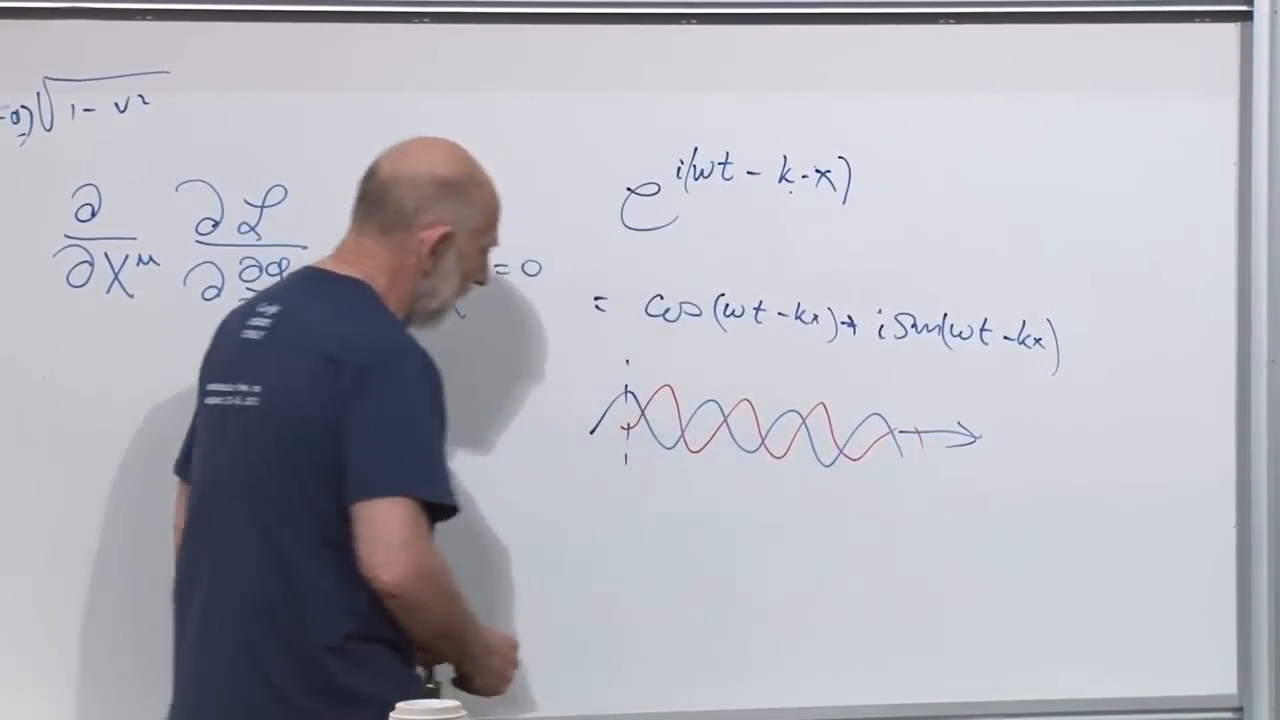
\includegraphics[width=0.90\textwidth]{lecture_05_figure_28.png}
\caption{余弦と正弦に分けられた複素平面波を、位相のずれた2つの実波として描いたもの。}
\lectureframe{01:56:00}
\end{figure}

\begin{classroomqa}
\audiencequestion{超伝導体中で電磁場が獲得する質量は、同じ種類の現象なのか。}
\lecturerresponse{密接に関係している：超伝導体では凝縮体が媒質中で電磁場に有効質量を与え、マイスナー効果を生じる。完全な説明には電磁場が必要であり、後回しにする。\lecturetimestamp{01:56:14}}
\end{classroomqa}

\begin{classroomqa}
\audiencequestion{ヒッグス機構は、ヒッグス粒子が空間を飛び回って質量を配って歩くものとして可視化できるのか。}
\lecturerresponse{いいえ。関係する対象はヒッグス場の背景値であり、個々のヒッグス粒子の流れではない。玩具的な作用では、背景は粒子の質量として機能する係数を変えるだけである。\lecturetimestamp{01:57:31}}
\end{classroomqa}

\begin{classroomqa}
\audiencequestion{同じスカラー背景への異なる結合が異なる質量を生みうるのか。}
\lecturerresponse{はい。ずれは結合 \(g\) に比例する。標準模型では、異なる湯川結合こそが、異なるフェルミオンが同じヒッグス背景から異なる質量を獲得する理由そのものである。\lecturetimestamp{01:58:04}}
\end{classroomqa}

\begin{classroomqa}
\audiencequestion{\(\phi\) 自体が質量項なのか。}
\lecturerresponse{この玩具模型では、\(g\phi_0\) はあらゆる力学的側面において質量係数への寄与として機能する。結合と背景値の両方を含めなければならない。\lecturetimestamp{01:58:42}}
\end{classroomqa}

\begin{classroomqa}
\audiencequestion{ヒッグス背景が消えたなら、すべての粒子は質量ゼロになるのか。}
\lecturerresponse{いいえ。電子、クォーク、弱ゲージボソンは通常の電弱質量への寄与を失い、ニュートリノの詳細はニュートリノに質量を与える機構に依存する。スカラー部門自体は、その背景値が消えるというだけで質量ゼロになる必要はない。陽子と中性子の質量の大部分は代わりにQCDの束縛と閉じ込めから来るので、ヒッグス場によって直接生成されるのではない。\lecturetimestamp{01:58:51}}
\end{classroomqa}

それでも原子への帰結は劇的である。ボーアスケールは自然単位で
\begin{equation}
a_0\sim\frac{1}{\alpha m_e}
\end{equation}
のように振る舞う。電子質量をゼロへ向かわせると、通常の原子長スケールは発散し、通常の局在した原子は存在しなくなる。陽子と中性子は、その質量が主に力学的なQCDエネルギーであるため、はるかに直接的には影響を受けないであろう。

これらの部分は今や一つの連続した議論を形成している。ローレンツ幾何学が観測される波長を支配する。一つの作用の中の一つの混合項が二つの力学系を互いに影響し合わせる。スカラー場は粒子に対するポテンシャルと、その粒子によって源を与えられる場の両方になる。計量と添字記法がローレンツ不変性を可視化し、最も単純な二次の不変密度がクライン--ゴルドン波を生み出す。最後に、一定のスカラー背景が同じ結合を質量のずれに変える。全体を通じての方法は、今後も持続するものである。すなわち、不変な作用を構成し、あらゆる力学的対象を変分し、得られた方程式から相互の物理を読み取るのである。